%                                                                 aa.dem
% AA vers. 9.1, LaTeX class for Astronomy & Astrophysics
% demonstration file
%                                                       (c) EDP Sciences
%-----------------------------------------------------------------------
%
% \documentclass[referee]{aa} % for a referee version
%\documentclass[onecolumn]{aa} % for a paper on 1 column  
%\documentclass[longauth]{aa} % for the long lists of affiliations 
%\documentclass[letter]{aa} % for the letters 
%\documentclass[bibyear]{aa} % if the references are not structured 
%                              according to the author-year natbib style

%

\documentclass{aa}  

%
\usepackage{graphicx}
\usepackage{amsmath,amsfonts,amssymb}
\usepackage{natbib}


%%%%%%%%%%%%%%%%%%%%%%%%%%%%%%%%%%%%%%%%
\usepackage{txfonts}
\usepackage{xcolor}

\usepackage{blindtext}
%%%%%%%%%%%%%%%%%%%%%%%%%%%%%%%%%%%%%%%%
% \usepackage[options]{hyperref}
% To add links in your PDF file, use the package "hyperref"
% with options according to your LaTeX or PDFLaTeX drivers.
\usepackage{float}
%\usepackage{stfloats}
\usepackage{dblfloatfix}
\usepackage{afterpage}
\usepackage{ifthen}
\usepackage[morefloats=12]{morefloats}

\usepackage{placeins}
\usepackage{multicol}
\usepackage[export]{adjustbox}\usepackage[breaklinks,colorlinks,citecolor=blue]{hyperref}
\bibpunct{(}{)}{;}{a}{}{,}
\usepackage[switch]{lineno}
\definecolor{linkcolor}{rgb}{0.6,0,0}
\definecolor{citecolor}{rgb}{0,0,0.75}
\definecolor{urlcolor}{rgb}{0.12,0.46,0.7}
%\usepackage[breaklinks, colorlinks, urlcolor=urlcolor,linkcolor=linkcolor,citecolor=citecolor,pdfencoding=auto]{hyperref}
\hypersetup{linktocpage}
\usepackage{bold-extra}
\usepackage{tabularx, booktabs}
\usepackage{amsmath}

%Planck style file, to be used with A&A style to produce Planck papers for publication.
%
% version 28 September 2010 --- useful macros --- CRL
% version 17 October 2010   --- first cut at important instrument values, from Daniele Mennella and
%                               Francois Bouchet, 13 October 2010 --- CRL
% version 18 October 2010   --- LFI FWHM changed to one value per feed, rather than M & S separately
%                               LFI FWHM uncertainties added for individual feeds.  Corrections made
%                               to LFI values. --- Andrea Zacchei
% version 24 October 2010   --- added to and corrected definitions.  No changes made to instrument
%                               quantities. --- CRL 
% version 31 October 2010   --- added definition of \muKHz. --- CRL
%
% version 15 November 2010  --- fixed conflict with aa.cls in definition of \endtable
%                               by naming the command below "\endPlancktable".  See section
%                               13.16 of the Style Guide.
%
% version 06 December 2010  --- Set up names with and without units.
%                               Add \allearlypapers command to ensure that all early papers are
%                               included in the reference list.
%                               Define macro for the name of the 4He JT cooler.
%
% version 07 December 2010  --- removed extraneous "planck2011-1.2" entry in \allearlypapers
%
% version 12 December 2010  --- added \endPlancktablewide command to set tablenotes to the full
%                               page width in the \begin{table*}...\end{table*} environment when
%                               the ``twocolumn'' option is specified in the \documentclass command.
%                               (It would be more elegant to extract the appropriate width from the
%                               aa.cls system at the time of execution, but that is buried more
%                               deeply in the system than I investigated.)
%
% version 05 January 2011   --- added unit \MJysr.  HFI performance values updated per FRB email
%                               01/05/2011 02:38-0800, and Brendan Crill email 01/05/2011 18:08 -0800.
%
% version 06 January 2011   --- changed \scriptscriptstyle primes to \scriptstyle, to better match the
%                               tx fonts used by A&A.
%
% version 07 January 2011   --- modified \allearlypapers to correspond with final early paper list.  
%                               Fixed 545 GHz center frequency.
%
% version 07 January 2011b  --- changed LFI white-noise sensitivity numbers to correct problem with units
%
% version 05 July 2011      --- added \Msol and \Lsol to get the symbols for solar mass and luminosity.
%                               Deleted previous definitions of \solar and \sol, which were equivalent
%                               to the new \Msol.
%
% version 16 August 2011    --- changed comments on \endPlancktable and \endPlancktablewide for clarity
%
% version 11 September 2011 --- changed definition of \tablenote to make footnote labels italic, as per A\&A
%
% version 26 April 2011     --- changed definition of \Planck to agree with what is said in the Style Guide (!)
%
% version 04 Dec 2013       --- included 2013 results references
%
% version 17 Jan 2014       --- included fix to bibtex file v4.3, i.e. \providecommand{\sorthelp}[1]{}
%
% version 26 Jul 2014       --- fixed incompatibility problem with aa.cls v8.0 and v8.2.  v8.2 should now be used
%                               for all Planck papers.
%                           --- fixed problem in definition of "\all2013resultspapers" that introduced a blanck
%                               into the reference to p06b.
%                           --- removed all the parameter definition stuff at the end.  We weren't using it, and
%                               it took up a lot of space.
%
% version 28 Jan 2015       --- added "\alltwentyfiftennresultspapers" and corrected "\all2013resultspapers" to
%                               "\all20thirteenresultspapers",
%
% Usage:  after the \documentclass[traditabstract]{aa} command in the La\TeX\ input file,
%         add this command:      \input Planck.tex


\def\setsymbol#1#2{\expandafter\def\csname #1\endcsname{#2}}
\def\getsymbol#1{\csname #1\endcsname}

%-----------------------------------------------------------------------
% Planck
%-----------------------------------------------------------------------
\def\Planck{\textit{Planck}}

%-----------------------------------------------------------------------
% The Planck Helium-4 JT cooler
%-----------------------------------------------------------------------
\def\HeJT{$^4$He-JT}

%-----------------------------------------------------------------------
% To include all Planck Early Results papers in the reference lists
%-----------------------------------------------------------------------
\def\allearlypapers{\nocite{planck2011-1.1, planck2011-1.3, planck2011-1.4, planck2011-1.5, planck2011-1.6, planck2011-1.7, planck2011-1.10, planck2011-1.10sup, planck2011-5.1a, planck2011-5.1b, planck2011-5.2a, planck2011-5.2b, planck2011-5.2c, planck2011-6.1, planck2011-6.2, planck2011-6.3a, planck2011-6.4a, planck2011-6.4b, planck2011-6.6, planck2011-7.0, planck2011-7.2, planck2011-7.3, planck2011-7.7a, planck2011-7.7b, planck2011-7.12, planck2011-7.13}}

%-----------------------------------------------------------------------
% To include all Planck 2013 Results papers in the reference lists
%-----------------------------------------------------------------------
\def\alltwentythirteenresultspapers{\nocite{planck2013-p01, planck2013-p02, planck2013-p02a, planck2013-p02d, planck2013-p02b, planck2013-p03, planck2013-p03c, planck2013-p03f, planck2013-p03d, planck2013-p03e, planck2013-p01a, planck2013-p06, planck2013-p03a, planck2013-pip88, planck2013-p08, planck2013-p11, planck2013-p12, planck2013-p13, planck2013-p14, planck2013-p15, planck2013-p05b, planck2013-p17, planck2013-p09, planck2013-p09a, planck2013-p20, planck2013-p19, planck2013-pipaberration, planck2013-p05, planck2013-p05a, planck2013-pip56, planck2013-p06b, planck2013-p01a}}

%-----------------------------------------------------------------------
% To include all Planck 2015 Results papers in the reference lists
%-----------------------------------------------------------------------
\def\alltwentyfifteenresultspapers{\nocite{planck2014-a01, planck2014-a03, planck2014-a04, planck2014-a05, planck2014-a06, planck2014-a07, planck2014-a08, planck2014-a09, planck2014-a11, planck2014-a12, planck2014-a13, planck2014-a14, planck2014-a15, planck2014-a16, planck2014-a17, planck2014-a18, planck2014-a19, planck2014-a20, planck2014-a22, planck2014-a24, planck2014-a26, planck2014-a28, planck2014-a29, planck2014-a30, planck2014-a31, planck2014-a35, planck2014-a36, planck2014-a37, planck2014-ES}}

%-----------------------------------------------------------------------
% Tables
%-----------------------------------------------------------------------
\newbox\tablebox    \newdimen\tablewidth
\def\leaderfil{\leaders\hbox to 5pt{\hss.\hss}\hfil}
%
% use the following definition of \endPlancktable for ApJ style notes to tables, set to the 
%         width of the table
% \def\endPlancktable{\tablewidth=\wd\tablebox 
%
% use the following definitions of \endPlancktable and \endPlancktablewide for A&A style notes 
% set to one-column  or full-page width, respectively
\def\endPlancktable{\tablewidth=\columnwidth 
    $$\hss\copy\tablebox\hss$$
    \vskip-\lastskip\vskip -2pt}
\def\endPlancktablewide{\tablewidth=\textwidth 
    $$\hss\copy\tablebox\hss$$
    \vskip-\lastskip\vskip -2pt}
\def\tablenote#1 #2\par{\begingroup \parindent=0.8em
    \abovedisplayshortskip=0pt\belowdisplayshortskip=0pt
    \noindent
    $$\hss\vbox{\hsize\tablewidth \hangindent=\parindent \hangafter=1 \noindent
    \hbox to \parindent{$^#1$\hss}\strut#2\strut\par}\hss$$
    \endgroup}
\def\doubleline{\vskip 3pt\hrule \vskip 1.5pt \hrule \vskip 5pt}

%-----------------------------------------------------------------------
% useful macros
%-----------------------------------------------------------------------
%
\def\L2{\ifmmode L_2\else $L_2$\fi}
%
\def\dtt{\Delta T/T}
\def\DeltaT{\ifmmode \Delta T\else $\Delta T$\fi}
\def\deltat{\ifmmode \Delta t\else $\Delta t$\fi}
\def\fknee{\ifmmode f_{\rm knee}\else $f_{\rm knee}$\fi}
\def\Fmax{\ifmmode F_{\rm max}\else $F_{\rm max}$\fi}
%
\def\solar{\ifmmode{\rm M}_{\mathord\odot}\else${\rm M}_{\mathord\odot}$\fi}
\def\Msolar{\ifmmode{\rm M}_{\mathord\odot}\else${\rm M}_{\mathord\odot}$\fi}
\def\Lsolar{\ifmmode{\rm L}_{\mathord\odot}\else${\rm L}_{\mathord\odot}$\fi}
%
\def\inv{\ifmmode^{-1}\else$^{-1}$\fi}
\def\mo{\ifmmode^{-1}\else$^{-1}$\fi}
\def\sup#1{\ifmmode ^{\rm #1}\else $^{\rm #1}$\fi}
\def\expo#1{\ifmmode \times 10^{#1}\else $\times 10^{#1}$\fi}
%
\def\,{\thinspace}
\def\lsim{\mathrel{\raise .4ex\hbox{\rlap{$<$}\lower 1.2ex\hbox{$\sim$}}}}
\def\gsim{\mathrel{\raise .4ex\hbox{\rlap{$>$}\lower 1.2ex\hbox{$\sim$}}}}
\let\lea=\lsim
\let\gea=\gsim
\def\simprop{\mathrel{\raise .4ex\hbox{\rlap{$\propto$}\lower 1.2ex\hbox{$\sim$}}}}
%
\def\deg{\ifmmode^\circ\else$^\circ$\fi}
\def\pdeg{\ifmmode $\setbox0=\hbox{$^{\circ}$}\rlap{\hskip.11\wd0 .}$^{\circ}
          \else \setbox0=\hbox{$^{\circ}$}\rlap{\hskip.11\wd0 .}$^{\circ}$\fi}
\def\arcs{\ifmmode {^{\scriptstyle\prime\prime}}
          \else $^{\scriptstyle\prime\prime}$\fi}
\def\arcm{\ifmmode {^{\scriptstyle\prime}}
          \else $^{\scriptstyle\prime}$\fi}
\newdimen\sa  \newdimen\sb
\def\parcs{\sa=.07em \sb=.03em
     \ifmmode \hbox{\rlap{.}}^{\scriptstyle\prime\kern -\sb\prime}\hbox{\kern -\sa}
     \else \rlap{.}$^{\scriptstyle\prime\kern -\sb\prime}$\kern -\sa\fi}
\def\parcm{\sa=.08em \sb=.03em
     \ifmmode \hbox{\rlap{.}\kern\sa}^{\scriptstyle\prime}\hbox{\kern-\sb}
     \else \rlap{.}\kern\sa$^{\scriptstyle\prime}$\kern-\sb\fi}
%
\def\ra[#1 #2 #3.#4]{#1\sup{h}#2\sup{m}#3\sup{s}\llap.#4}
\def\dec[#1 #2 #3.#4]{#1\deg#2\arcm#3\arcs\llap.#4}
\def\deco[#1 #2 #3]{#1\deg#2\arcm#3\arcs}
\def\rra[#1 #2]{#1\sup{h}#2\sup{m}}
%
\def\page{\vfill\eject}
\def\dots{\relax\ifmmode \ldots\else $\ldots$\fi}
%
%-----------------------------------------------------------------------
% units
%-----------------------------------------------------------------------
%
\def\WHzsr{\ifmmode $W\,Hz\mo\,sr\mo$\else W\,Hz\mo\,sr\mo\fi}
\def\mHz{\ifmmode $\,mHz$\else \,mHz\fi}
\def\GHz{\ifmmode $\,GHz$\else \,GHz\fi}
\def\mKs{\ifmmode $\,mK\,s$^{1/2}\else \,mK\,s$^{1/2}$\fi}
\def\muKs{\ifmmode \,\mu$K\,s$^{1/2}\else \,$\mu$K\,s$^{1/2}$\fi}
\def\muKRJs{\ifmmode \,\mu$K$_{\rm RJ}$\,s$^{1/2}\else \,$\mu$K$_{\rm RJ}$\,s$^{1/2}$\fi}
\def\muKHz{\ifmmode \,\mu$K\,Hz$^{-1/2}\else \,$\mu$K\,Hz$^{-1/2}$\fi}
\def\MJysr{\ifmmode \,$MJy\,sr\mo$\else \,MJy\,sr\mo\fi}
\def\MJysrmK{\ifmmode \,$MJy\,sr\mo$\,mK$_{\rm CMB}\mo\else \,MJy\,sr\mo\,mK$_{\rm CMB}\mo$\fi}
\def\microns{\ifmmode \,\mu$m$\else \,$\mu$m\fi}
\def\micron{\microns}
\def\muK{\ifmmode \,\mu$K$\else \,$\mu$\hbox{K}\fi}
\def\microK{\ifmmode \,\mu$K$\else \,$\mu$\hbox{K}\fi}
\def\muW{\ifmmode \,\mu$W$\else \,$\mu$\hbox{W}\fi}
\def\kms{\ifmmode $\,km\,s$^{-1}\else \,km\,s$^{-1}$\fi}
\def\kmsMpc{\ifmmode $\,\kms\,Mpc\mo$\else \,\kms\,Mpc\mo\fi}
%
%
%----------------------------------------------------------------------
% set up machinery to list Planck papers in roman numeral order.
%----------------------------------------------------------------------

\providecommand{\sorthelp}[1]{}


\def\commander{\texttt{Commander}}
\def\commanderone{\texttt{Commander1}}
\def\commandertwo{\texttt{Commander2}}
\def\commanderthree{\texttt{Commander3}}


\newcommand{\phm}{\phantom{-}}
\newcommand{\dv}[0]{\vec{d}}
\renewcommand{\t}[0]{\vec{t}}
\newcommand{\A}[0]{\tens{A}}
\newcommand{\B}[0]{\mathrm{B}}
\newcommand{\Y}[0]{\tens{Y}}
\newcommand{\n}[0]{\vec{n}}
\newcommand{\red}[0]{\color{red}}
\newcommand{\green}[0]{\color{green}}
\newcommand{\s}[0]{\vec{s}}
\renewcommand{\a}[0]{\vec{a}}
\newcommand{\m}[0]{\vec{m}}
\newcommand{\bv}[0]{\vec{b}}
\newcommand{\f}[0]{\vec{f}}
\newcommand{\F}[0]{\tens{F}}
\newcommand{\T}[0]{\tens{T}}
\newcommand{\Cp}[0]{\tens{C}}
\renewcommand{\L}[0]{\tens{L}}
\newcommand{\g}[0]{\vec{g}}
\newcommand{\N}[0]{\tens{N}}
\newcommand{\M}[0]{\tens{M}}
\newcommand{\iN}[0]{\tens{N}^{-1}}
\newcommand{\iM}[0]{\tens{M}^{-1}}
\newcommand{\w}[0]{\vec{w}}
\renewcommand{\S}[0]{\tens{S}}
\renewcommand{\r}[0]{\vec{r}}
\renewcommand{\u}[0]{\vec{u}}
\newcommand{\q}[0]{\vec{q}}
\renewcommand{\v}[0]{\vec{v}}
\renewcommand{\P}[0]{\tens{P}}
\newcommand{\dt}[0]{d_t}
\newcommand{\di}[0]{d_i}
\newcommand{\nt}[0]{n_t}
\newcommand{\st}[0]{s_t}
\newcommand{\mt}[0]{m_t}
\newcommand{\ft}[0]{f_t}
\newcommand{\Te}[0]{T_{\rm e}}
\newcommand{\EM}[0]{\rm EM}
\newcommand{\hi}{\ensuremath{\mathsc {Hi}}}
\newcommand{\bpbold}{\bfseries{\scshape{BeyondPlanck}}}
\newcommand{\BP}{\textsc{BeyondPlanck}}
\newcommand{\bp}{\textsc{BeyondPlanck}}
\newcommand{\cosmoglobe}{\textsc{Cosmoglobe}}
\newcommand{\Cosmoglobe}{\textsc{Cosmoglobe}}
\newcommand{\lfi}[0]{LFI}
\newcommand{\hfi}[0]{HFI}
\newcommand{\npipe}[0]{\texttt{NPIPE}}
\newcommand{\K}[0]{\textit K}
\newcommand{\Ka}[0]{\textit{Ka}}
\newcommand{\Q}[0]{\textit Q}
\newcommand{\V}[0]{\textit V}
\newcommand{\W}[0]{\textit W}
\newcommand{\e}{\mathrm e}
\newcommand{\cvar}{\ensuremath{c(\vartheta, \varphi, \psi)}}


% Custom definitions
\newcommand{\mathsc}[1]{{\normalfont\textsc{#1}}}
\def\Cosmoglobe{\textsc{Cosmoglobe}}
\def\Planck{\textit{Planck}}
\def\WMAP{\textit{WMAP}}

\newcolumntype{C}{>{\centering\arraybackslash}m{0.3\textwidth}}

\newcolumntype{B}{>{\centering\arraybackslash}m{0.03\textwidth}}


\begin{document} 


   \title{$N+2$ mapmaking for polarized CMB experiments}

   %This author list corresponds to \title{Author list for L04\_CMB\_Foregrounds\_Extraction}
%Prepared by M. Lopez-Caniego (Marcos.Lopez.Caniego@sciops.esa.int), ESAC/ESA
%This version is from Thu Jul 12 18:11:48 2018 CET
%\subtitle{There are 152 co-authors in this list}
\newcommand{\oslo}[0]{1}
\newcommand{\iiabangalore}[0]{2}

\author{\small
D.~J.~Watts\inst{\ref{uio}}\thanks{Corresponding author: D.~J.~Watts; \url{duncanwa@astro.uio.no}}
\and
A.~Basyrov\inst{\ref{uio}}
\and
H.~T.~Ihle\inst{\ref{uio}}
\and
S.~Paradiso\inst{\ref{waterloo}}
\and
F.~Rahman\inst{\ref{iiabangalore}}
\and
H.~Thommesen\inst{\ref{uio}}
\and
M.~Bersanelli\inst{\ref{milan}}
\and
L.~A.~Bianchi\inst{\ref{milan}}
\and
M.~Brilenkov\inst{\ref{uio}}
\and
L.~P.~L.~Colombo\inst{\ref{milan}}
\and
H.~K.~Eriksen\inst{\ref{uio}}
\and
J.~R.~Eskilt\inst{\ref{uio},\ref{imperial}}
\and
K.~S.~F.~Fornazier\inst{\ref{saopaulo}}
\and
C.~Franceschet\inst{\ref{milan}}
\and
U.~Fuskeland\inst{\ref{uio}}
\and
M.~Galloway\inst{\ref{uio}}
\and
E.~Gjerl\o w\inst{\ref{uio}}
\and
B.~Hensley\inst{\ref{princeton}}
\and
L.~T.~Hergt\inst{\ref{ubc}}
\and
D.~Herman\inst{\ref{uio}}
\and
G.~A.~Hoerning\inst{\ref{saopaulo}}
\and
K.~Lee\inst{\ref{uio}}
\and
J.~G.~S.~Lunde\inst{\ref{uio}}
\and
A.~Marins\inst{\ref{saopaulo},\ref{ustofc}}
\and
S.~K.~Nerval\inst{\ref{dunlap1},\ref{dunlap2}}
\and
S.~K.~Patel\inst{\ref{iit_bhu}}
\and
M.~Regnier\inst{\ref{apc}}
\and
M.~San\inst{\ref{uio}}
\and
S.~Sanyal\inst{\ref{iit_bhu}}
\and
N.-O.~Stutzer\inst{\ref{uio}}
\and
A.~Verma\inst{\ref{iit_bhu}}
\and
I.~K.~Wehus\inst{\ref{uio}}
\and
Y.~Zhou\inst{\ref{berkeley}}
}
\institute{\small
Institute of Theoretical Astrophysics, University of Oslo, Blindern, Oslo, Norway\label{uio}
\and
Waterloo Centre for Astrophysics, University of Waterloo, Waterloo, ON N2L 3G1, Canada\label{waterloo}
\and
Indian Institute of Astrophysics, Koramangala II Block, Bangalore, 560034, India\label{iiabangalore}
\and
Dipartimento di Fisica, Università degli Studi di Milano, Via Celoria, 16, Milano, Italy\label{milan}
\and
Imperial Centre for Inference and Cosmology, Department of Physics, Imperial College London, Blackett Laboratory, Prince Consort Road, London SW7 2AZ, United Kingdom\label{imperial}
\and
Instituto de Física, Universidade de São Paulo - C.P. 66318, CEP: 05315-970, São Paulo, Brazil\label{saopaulo}
\and
Department of Astrophysical Sciences, Princeton University, 4 Ivy Lane, Princeton, NJ 08540\label{princeton}
\and
Department of Physics and Astronomy, University of British Columbia, 6224 Agricultural Road, Vancouver BC, V6T1Z1, Canada\label{ubc}
\and
Department of Astronomy,  University of Science and Technology of China, Hefei, China\label{ustofc}
\and
David A. Dunlap Department of Astronomy \& Astrophysics, University of Toronto, 50 St. George Street, Toronto, ON M5S 3H4, Canada\label{dunlap1}
\and
Dunlap Institute for Astronomy \& Astrophysics, University of Toronto, 50 St. George Street, Toronto, ON M5S 3H4, Canada\label{dunlap2}
\and
Department of Physics, Indian Institute of Technology (BHU), Varanasi - 221005, India\label{iit_bhu}
\and
Laboratoire Astroparticule et Cosmologie (APC), Université Paris-Cité, Paris, France\label{apc}
\and
Department of Physics, UC Berkeley\label{berkeley}
}

 %\author{V.~Arsenijevic\inst{\ref{inst1}}\and S.~Fabbro\inst{\ref{inst2}}\and
%A.~M.~Mour\~ao\inst{\ref{inst3}}\and A.~J.~Rica da Silva\inst{\ref{inst1}}}
%
%\institute{Multidisciplinar de Astrof\'{\i}sica, IST, Avenida Rovisco Pais, 1049
%Lisbon, Portugal\email{...}\label{inst1} \and < Multidisciplinar de Astrof\'{\i}sica, IST, Avenida Rovisco Pais, 1049 Lisbon, Portugal\email{...}\label{inst2}
%\and
%Multidisciplinar de Astrof\'{\i}sica, IST, Avenida Rovisco Pais, 1049
%Lisbon, Portugal\email{...}\label{inst3}
%} 


   %\institute{Institute of Theoretical Astrophysics, University of Oslo, Blindern, Oslo, Norway}
  
   % Shortened title, author list for top of page 
   \titlerunning{$N+2$ mapmaking}
   \authorrunning{Galloway et al.}

   \date{\today} 
   
   \abstract{We introduce $N+2$ mapmaking as a novel approach to constructing maps in both intensity and polarization for multi-detector CMB data. The motivation behind this method is two-fold: Firstly, it provides individual temperature detector maps from a multi-detector set, which may be useful for component separation purposes, in particular for line emission reconstruction. Secondly, it simultaneously outputs coadded polarization maps with minimal temperature-to-polarization leakage sensitivity. Algorithmically speaking, the $N+2$ mapmaker is closely related to the `spurious mapmaking' algorithm pioneered by the \WMAP\ team, but rather than solving for a spurious $S$ map together with the three normal Stokes $IQU$ parameters, we solve for $N$ temperature maps and two Stokes ($Q$ and $U$) parameters per pixel. The result is a statistically coherent set of physically meaningful per-detector temperature maps, each with slightly different bandpasses as defined by each detector, combined with coadded polarization maps. We test this approach on \Planck\ Low Frequency Instrument (LFI) 30 GHz data, and unfortunately find that the \Planck\ scanning strategy is too poorly cross-linked to allow for a clean separation between temperature and polarization. However, noting that pairs of detectors within a single horn are strongly anti-correlated, we anticipate that solving for horn maps, as opposed to individual detector maps, may provide an optimal compromise between noise and temperature-to-polarization leakage minimization. When applied to simulated data with a rotating half-wave plate, for which the polarization angle coverage is greatly improved, the algorithm performs as expected. For such experiments, the $N+2$ mapmaker offers the option of constructing multi-detector maps with minimal temperature-to-polarization leakage, which potentially can be useful for detecting and mitigating low-level systematic effects. We conclude that $N+2$ mapmaking is a useful tool for adjusting the granularity of the temperature map decomposition of a given experiments, while still producing joint high signal-to-noise ratio polarization maps with minimal temperature-to-polarization leakage.
   }
   
   \maketitle
%\setcounter{tocdepth}{2}
%\tableofcontents
   
% INTRODUCTION
%-------------------------------------------------------------------
\section{Introduction}

The problem of bandpass mismatch is important when combining multiple Cosmic Microwave Background (CMB) detectors into a single polarization map \citep[e.g.,][]{page:2007,lfi2015,BP09}. Small differences in the bandpass of individual detectors can result in major disagreements about signal amplitudes in regions with bright foregrounds with non-thermal spectra, as each detector effectively observes a different sky signal. These disagreements then lead to temperature-to-polarization leakage as the differences in temperature are incorrectly interpreted as a polarized signal instead of as bandpass differences by the mapmaking algorithm. Experiments with bright line emission, for instance the rotational CO lines at multiples of 115\,GHz, are particularly sensitive to such bandpass mismatch effects \citep[e.g.,][]{hfi_processing:2013}. 

Multiple approaches have been proposed to mitigate this issue. The most obvious is to bin each detector independently in a separate map. However, this requires a sufficiently cross-linked scanning strategy, and in practice this approach is often only possible for experiments with a spinning half-wave plate that explicitly decouples the temperature and polarization signals in every single pixel \citep[e.g.,][]{abs:2016}. For poorly cross-linked scanning strategies, individual detector maps are usually not usable on their own, but rather require combination after the fact. Another common approach is to explicitly correct for the bandpass of each detector with respect to an explicit sky model that describes the spectral energy density of each component \citep[e.g.,][]{planck_fg:2015}, and subtract the predicted bandpass differences for each detector, either in terms of spatial templates \citep[e.g.,][]{lfi2015} or directly the level of time-ordered data \citep{bp01}. A third approach is to solve for an additional so-called `spurious map' together with the regular Stokes parameters, by adding an additional component to the mapmaking vector that accounts for the extra signal seen by an individual detector \citep{spurious}, at the cost of an increased conditional number in the mapmaking equation, and thereby somewhat higher noise. A fourth approach is to combine the latter two methods, by adjusting the bandpasses used in the explicit modelling approach by minimizing the amplitudes of the spurious maps \citep{BP09}.

In this paper, we introduce another variation that is closely inspired by the spurious mapmaking algorithm. However, rather than solving for one common temperature map and $N-1$ spurious maps, where $N$ denotes the number of detectors, we solve directly for $N$ individual temperature maps. We call this $N+2$ mapmaking, as it simply amounts to expanding the pointing matrix and the data vector in the mapmaking equation to produce single-detector intensity maps while simultaneously producing combined polarization maps for the entire frequency channel. This allows for the exact temperature bandpass to be used, while at the same time combining the polarization data to maximize the signal-to-noise ratio and minimize leakage effects. A main advantage of this approach over the traditional spurious mapmaking approach as described by \citet{spurious} is that it retains more foreground information to be used in higher-level analysis, and having direct access to individual detector or detector-set maps is particularly important for experiments with bright line emission, such as \Planck\ HFI \citep{planck_co:2014}. Indeed, preparing for a future end-to-end Bayesian analysis of the HFI data, similar to those already performed for LFI \citep{bp01}, \WMAP \citep{watts2023_dr1}, and DIRBE \citep{CG02_01} by the \bp\ and \Cosmoglobe\footnote{\url{http://cosmoglobe.uio.no}} collaborations, was the original motivation for the current work.  

We test this algorithm on real \Planck\ 30\,GHz data, and find that the \Planck\ scanning strategy is not sufficiently cross-linked to support a robust polarization reconstruction. To partially mitigate this problem, we consider the case of depolarized mapmaking \citep[e.g.,][]{npipe}, in which we first solve for common temperature and polarization maps; subtract the resulting projected polarization signals from the original time-ordered data; and re-solve for individual detector temperature maps. We finally test the $N+2$ mapmaking algorithm on a simulated data set that corresponds to the \Planck\ 30\,GHz measurements, but with an additional spinning half-wave plate.  

Section~\ref{sec:mapmaking} describes the problem and the mathematics of $N+2$ mapmaking. Section~\ref{sec:lfi} then describes the analysis pipeline and the application of this approach to \Planck\ LFI. Section~\ref{sec:depol} describes the case of depolarized mapmaking, and Sect.~\ref{sec:sim} demonstrates the full $N+2$ mapmaking procedure on simulated LFI data with a spinning half-wave plate. Finally, we conclude in Sect.~\ref{sec:conclusions}, and offer some avenues to exploit this technique in the future.

\begin{figure*}[p]
  \centering
  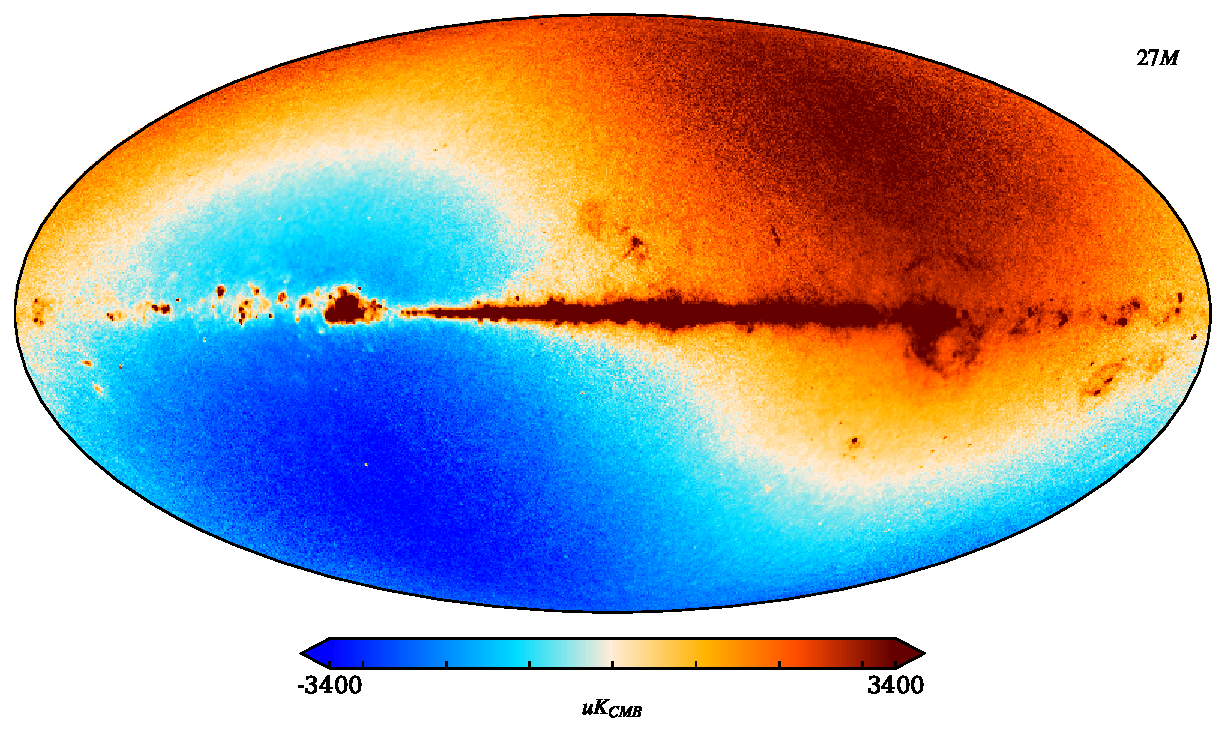
\includegraphics[width=0.48\textwidth]{figs/map_T_27M.pdf}
  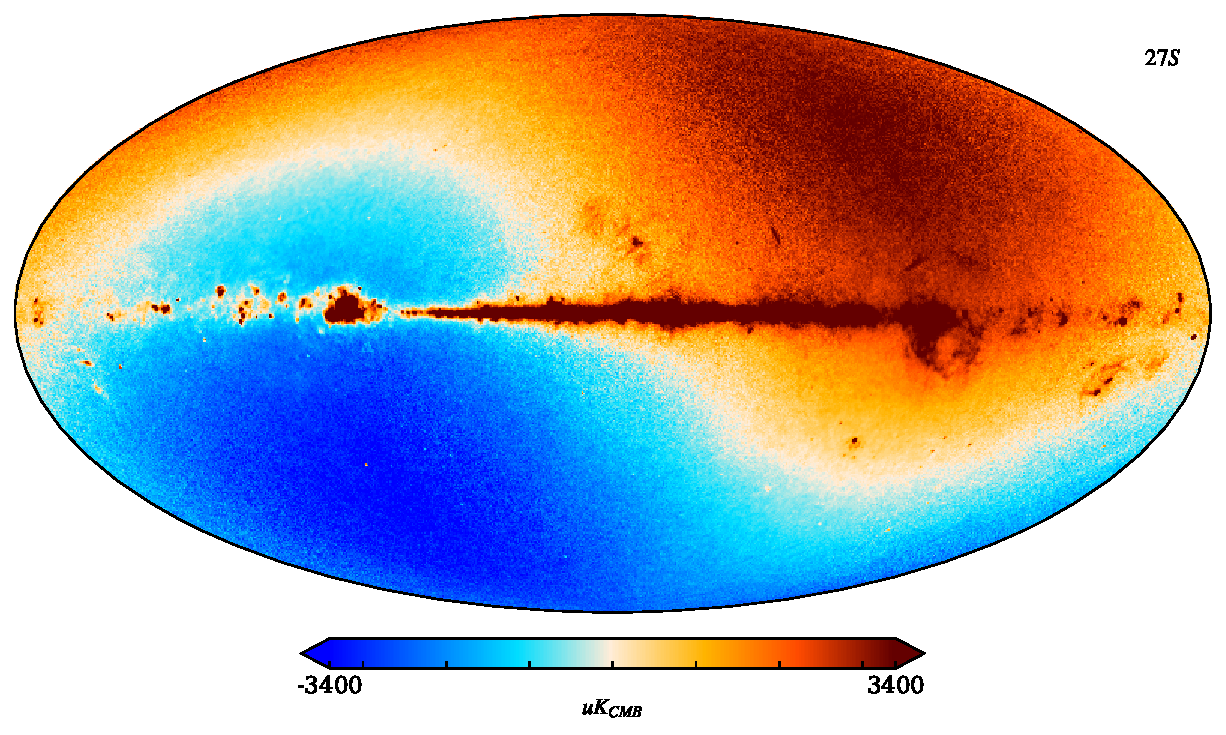
\includegraphics[width=0.48\textwidth]{figs/map_T_27S.pdf}\\
  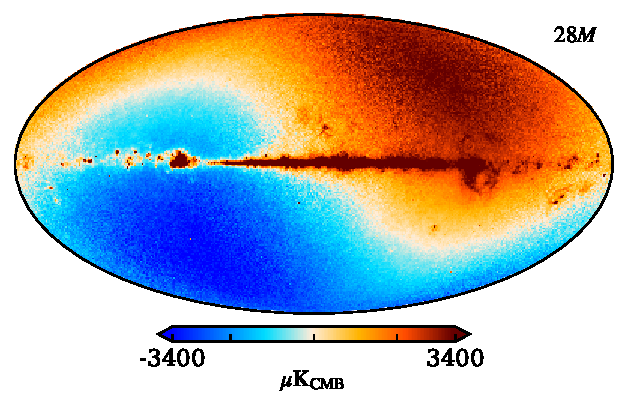
\includegraphics[width=0.48\textwidth]{figs/map_T_28M.pdf}
  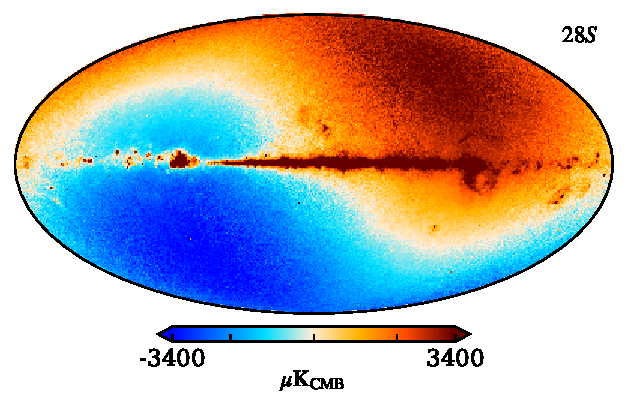
\includegraphics[width=0.48\textwidth]{figs/map_T_28S.pdf}\\
  %\includegraphics[width=0.5\columnwidth]{figs/cbar_temp.pdf}\\
  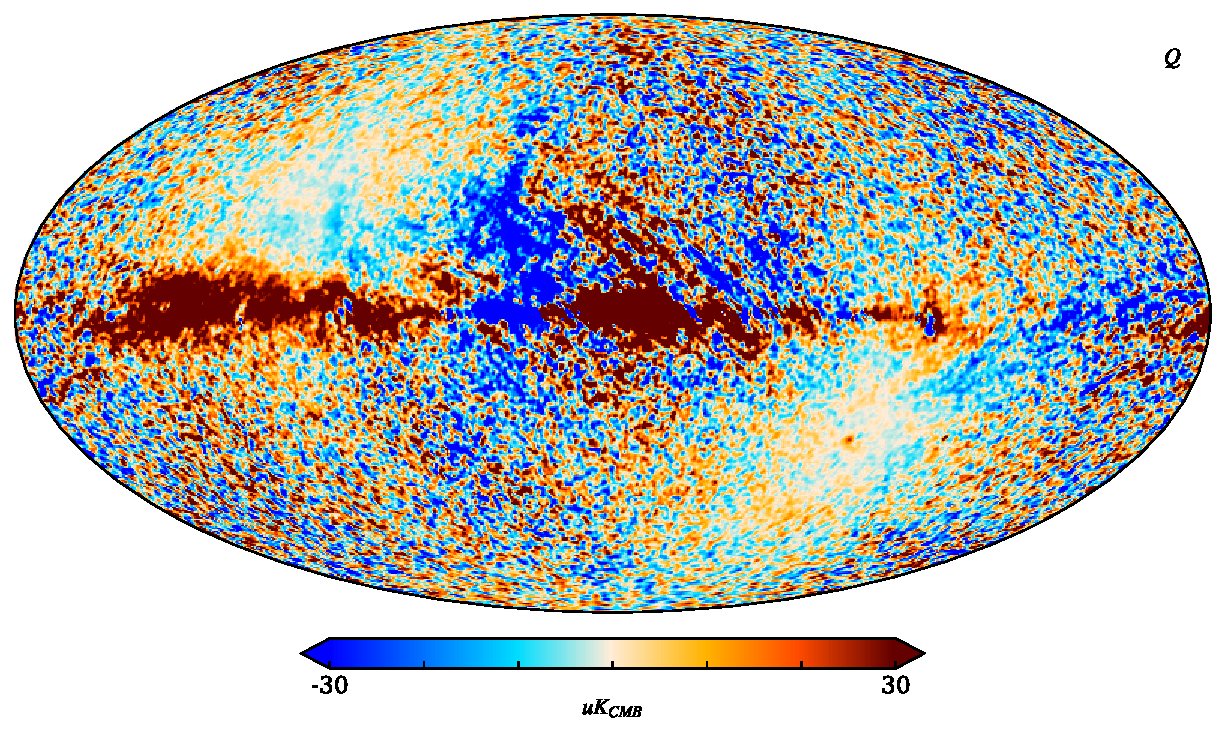
\includegraphics[width=0.48\textwidth]{figs/map_Q_badpol.pdf}
  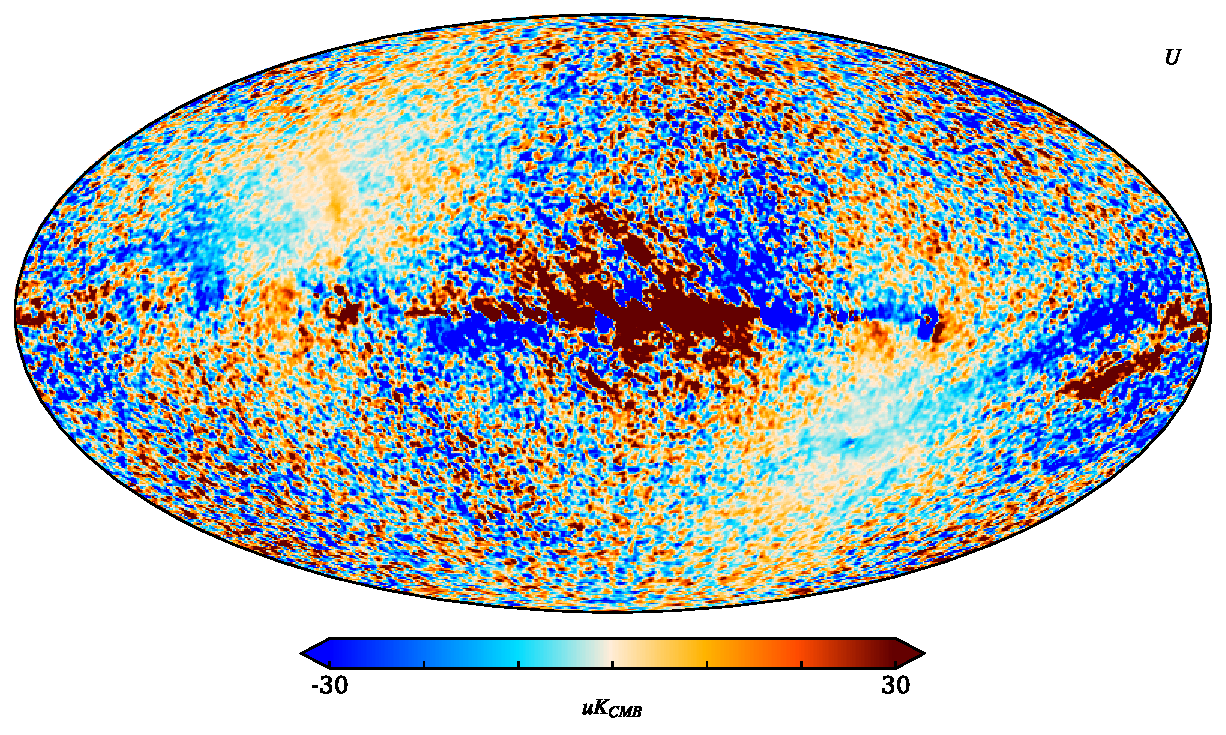
\includegraphics[width=0.48\textwidth]{figs/map_U_badpol.pdf}\\
  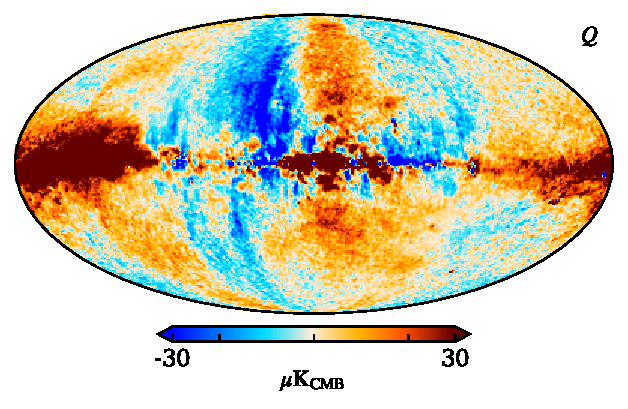
\includegraphics[width=0.48\textwidth]{figs/map_Q_binned.pdf}
  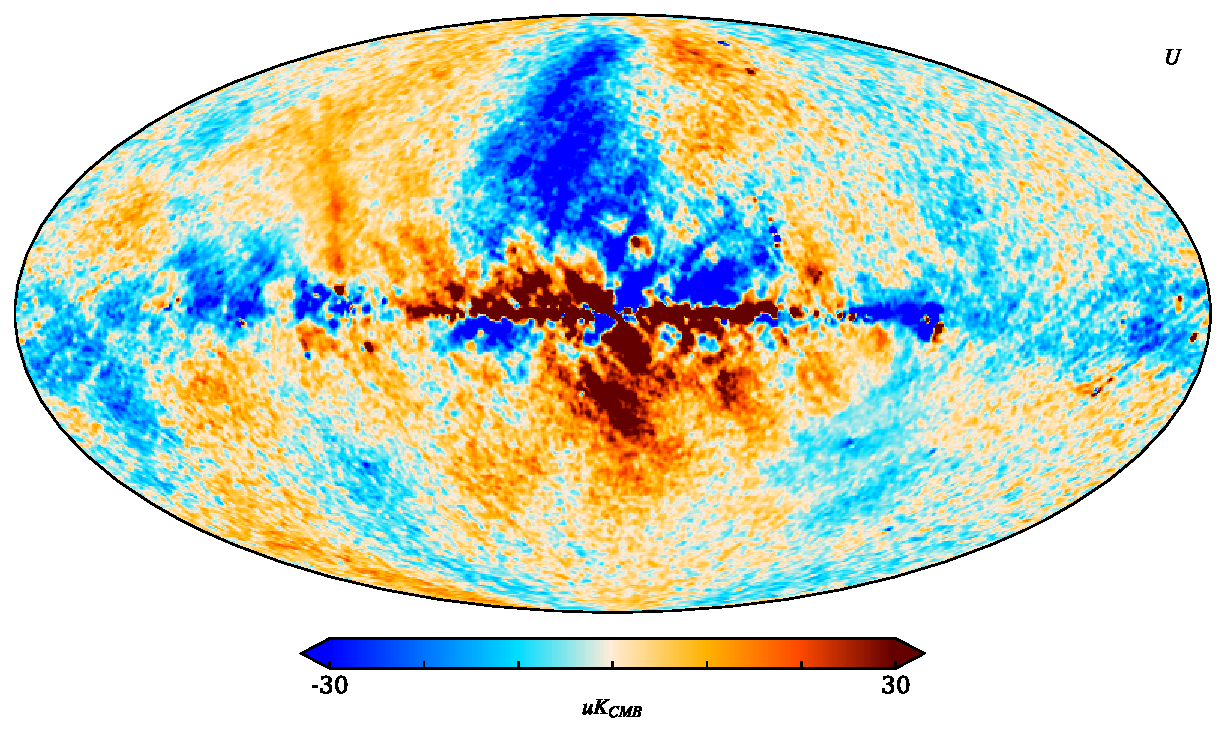
\includegraphics[width=0.48\textwidth]{figs/map_U_binned.pdf}\\
  %\includegraphics[width=0.5\columnwidth]{figs/cbar_pol.pdf}\\
  \caption{Temperature and polarization maps for the LFI 30\,GHz data produced using $N+2$ mapmaking. The top four panels shows temperature maps for individual detectors, and the third row shows the combined $Q$ and $U$ maps. The bottom row shows corresponding $Q$ and $U$ maps produced from a traditional binned mapmaker that co-adds all data into a common temperature map.}
  \label{fig:maps}
\end{figure*}


\section{Mathematical Description}
\label{sec:mapmaking}

The mapmaking problem is often expressed in the literature as \citep[e.g.,][]{de_Gasperis_2005}
\begin{equation}
d_t = \A_{t,p}s_p + n_t,
\end{equation}
where $t$ and $p$ denote time sample and pixel, respectively; $d_t$ is the detector timestream; $\A$ is the pointing matrix; $s$ is the signal vector; and $n$ represents zero-mean instrumental Gaussian noise with covariance $\N$. In the case of $N+2$ mapmaking, we write $d_t$ as 
\begin{equation}
d_t = \begin{pmatrix}
d_t^1\\ d_t^2\\ \vdots \\ d_t^i\\
\end{pmatrix},
\end{equation}
where $i$ indexes detectors, while the sky signal for a single pixel, $s_p$, is written as
\begin{equation}
s_p = \begin{pmatrix}
I_{1,p}\\
I_{2,p}\\
\vdots\\
I_{i,p}\\
Q_p\\
U_p\\
\end{pmatrix}.
\end{equation}
This differs from the standard approach by allowing individual temperature maps per detector. Our data model for the timestream of a single detector $i$ then becomes
\begin{equation}
d_{i,p,t} = I_{i,p} + Q_p \cos2\phi_i(t) + U_p \sin2\phi_i(t).
\label{eq:datamodel}
\end{equation}
The $Q$ and $U$ terms are in this model common between all detectors, and thus independent of $i$.

Based on this model, we generalize the pointing matrix such that it maps the correct detector to the correct temperature map,
\begin{equation}
\A_{t,p} = \begin{pmatrix}
1 & 0 & \cdots & 0 & \cos2\phi_1 & \sin2\phi_1 \\
0 & 1 & \cdots & 0 & \cos2\phi_2 & \sin2\phi_2 \\
\vdots & \vdots & \ddots & \vdots & \vdots & \vdots \\
0 & 0 & \cdots & 1 & \cos2\phi_i & \sin2\phi_i \\
\end{pmatrix},
\end{equation}
where, for notational ease, we have dropped the explicit function of time for the polarization angles. The standard Generalized Least Squares (GLS) solution to the mapmaking equation is as usual given by
\begin{equation}
\tilde{s}_p = (\A^t \N^{-1}\A)^{-1} \A^t\N^{-1}d.
\label{eq:gls}
\end{equation}


During the mapmaking process, we must accumulate the quantity $\A^t\N^{-1}\A$. Assuming $\N$ to be diagonal and given by
\begin{equation}
N = \begin{pmatrix}
\sigma^2_1 & 0 & \cdots & 0 \\
0 & \sigma^2_2 & \cdots & 0 \\
\vdots & \vdots & \ddots & \vdots \\
0 & 0 & \cdots & \sigma^2_i \\
\end{pmatrix},
\end{equation}
this quantity expands into
\begin{equation*}
\begin{tiny}
\sum_t
\begin{pmatrix}
(\frac{1}{\sigma_1})^2 & 0 & \cdots &
(\frac{1}{\sigma_1})^2 \cos2\phi_1 & (\frac{1}{\sigma_1})^2 \sin2\phi_1 \\

0 & (\frac{1}{\sigma_2})^2 & \cdots &
(\frac{1}{\sigma_2})^2 \cos2\phi_2 & (\frac{1}{\sigma_2})^2 \sin2\phi_2 \\

\vdots & \vdots & \ddots & \vdots & \vdots \\

(\frac{1}{\sigma_1})^2 \cos2\phi_1 & (\frac{1}{\sigma_2})^2 \cos2\phi_2 & \cdots & 
\sum_{i} (\frac{\cos 2\phi_i}{\sigma_i})^2 & \sum_{i} \frac{\sin2\phi_t \cos2\phi_i}{\sigma_i^2}  \\

(\frac{1}{\sigma_1})^2 \sin2\phi_1 & (\frac{1}{\sigma_2})^2 \sin2\phi_2 & \cdots &
\sum_{i} \frac{\sin2\phi_i \cos2\phi_i}{\sigma_i^2}  & \sum_{i} (\frac{ \sin 2\phi_i}{\sigma_i})^2
\\
\end{pmatrix}
\end{tiny}
\end{equation*}
for a given pixel, where the sum over $t$ represents the sum over all observation hitting a particular pixel $p$. Simultaneously, we can also accumulate the vector $\A^t\N^{-1}d$ which has the form
\begin{equation}
\sum_t
\begin{pmatrix}
\frac{d_{1}}{\sigma_1^2} \\
\frac{d_{2}}{\sigma_2^2}\\
\vdots\\
\frac{d_{i}}{\sigma_i^2}\\
\sum_i \frac{d_{i}}{\sigma_i^2} \cos2\phi_i\\
\sum_i \frac{d_{i}}{\sigma_i^2} \sin2\phi_i\\
\end{pmatrix}.
\end{equation}
Once these quantities are computed for all observations over the entire mission, it remains to simply invert the first matrix and front multiply the data vector to obtain the sky vector $\tilde{s}$, as described by Eq.~\ref{eq:gls}.

\begin{figure}[t]
  \centering
  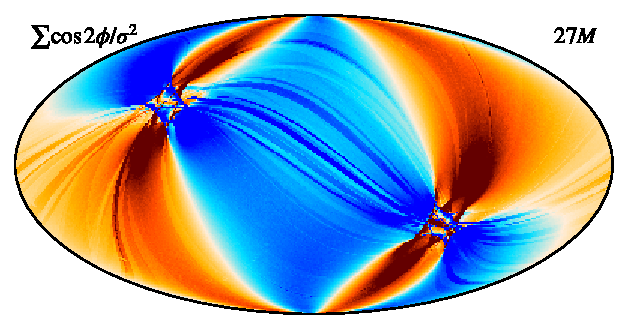
\includegraphics[width=0.47\linewidth]{figs/map_Q_polang27M.pdf}
  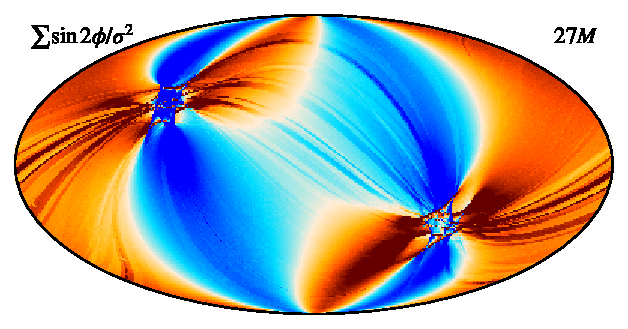
\includegraphics[width=0.47\linewidth]{figs/map_U_polang27M.pdf}\\
  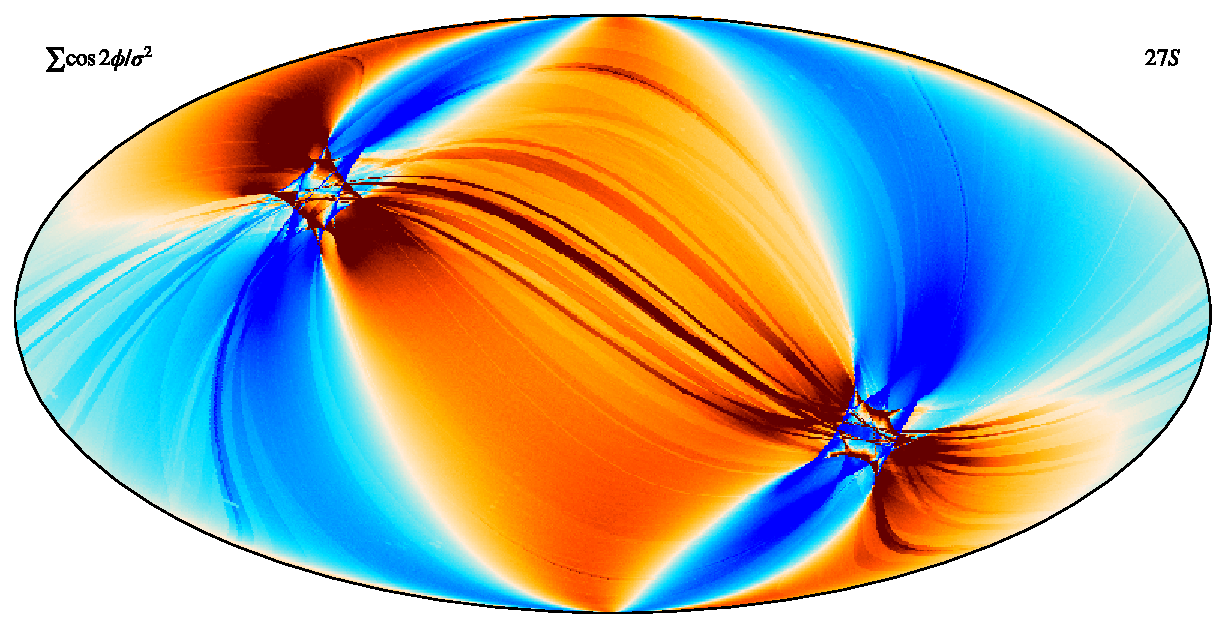
\includegraphics[width=0.47\linewidth]{figs/map_Q_polang27S.pdf}
  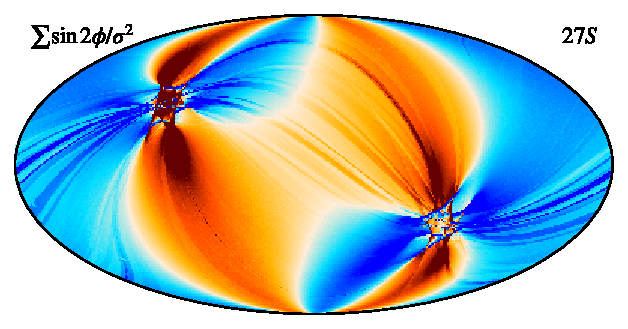
\includegraphics[width=0.47\linewidth]{figs/map_U_polang27S.pdf}\\
  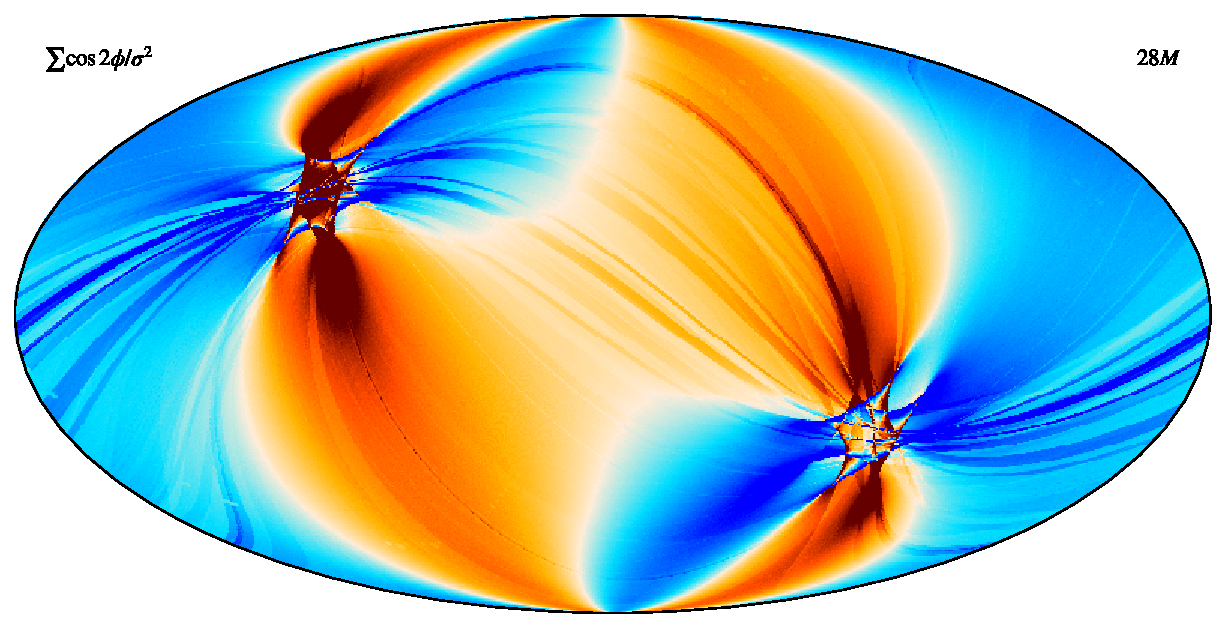
\includegraphics[width=0.47\linewidth]{figs/map_Q_polang28M.pdf}
  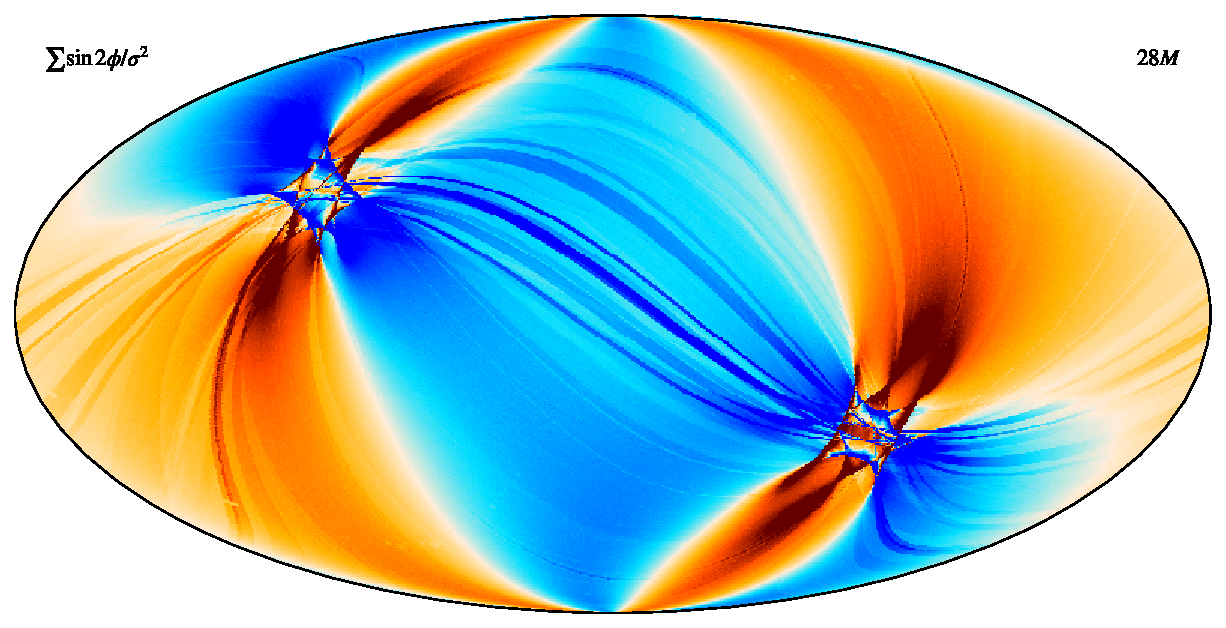
\includegraphics[width=0.47\linewidth]{figs/map_U_polang28M.pdf}\\
  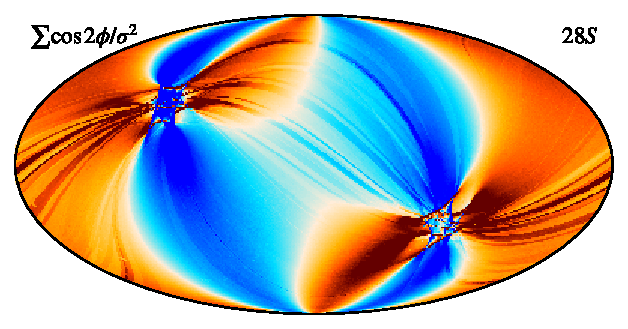
\includegraphics[width=0.47\linewidth]{figs/map_Q_polang28S.pdf}
  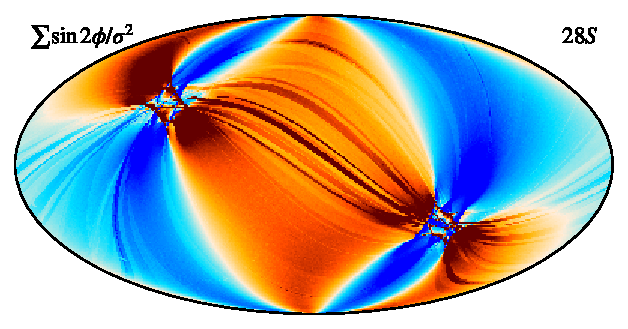
\includegraphics[width=0.47\linewidth]{figs/map_U_polang28S.pdf}\\
  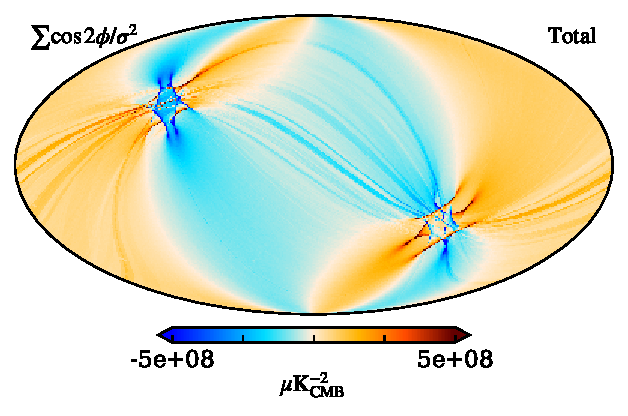
\includegraphics[width=0.47\linewidth]{figs/map_Q_polang_all.pdf}
  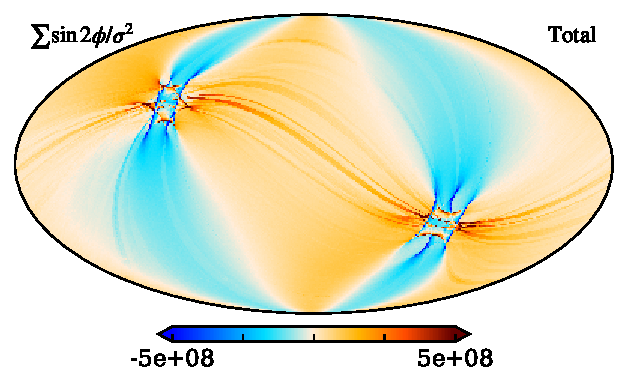
\includegraphics[width=0.47\linewidth]{figs/map_U_polang_all.pdf}\\
  %\includegraphics[width=0.5\columnwidth]{figs/cbar_pol.pdf}\\
  \caption{Polarization terms from the four 30\,GHz LFI detectors (rows 1--4) and the combined term used by the traditional binned mapmaker (bottom row). The left column shows the Stokes $Q$ term $(\frac{1}{\sigma})^2 \cos2\phi$, and the right column shows the Stokes $U$ term, $(\frac{1}{\sigma})^2 \sin2\phi$.}
  \label{fig:polangles}
\end{figure}


%Traditional polarized mapmaking for CMB experiments uses a matrix that looks like this (for a given timestep omitting all other columns):

%\begin{equation}
%M = \begin{pmatrix} 
%1          & cos(2\phi) & sin(2\phi)\\
%cos(2\phi) & cos^2(2\phi) & sin(2\phi) cos(2\phi) \\
%sin(2\phi) & sin(2\phi) cos(2\phi) & sin^2(2\phi) \\ 
%  \end{pmatrix}
%\end{equation}

%For n+2 mapmaking, we can generalize it to look like this

%\begin{equation}
%M = \begin{pmatrix} 
%\delta_d & 0 & \cdots  & \delta_d cos(2\phi) & \delta_d sin(2\phi)\\
%0 & \delta_d & \cdots  & \delta_d cos(2\phi) & \delta_d sin(2\phi)\\
%\vdots & \vdots & \ddots & \vdots & \vdots \\
%\delta_d cos(2\phi) & \delta_d cos(2\phi) & \cdots  & cos^2(2\phi) & sin(2\phi) cos(2\phi) \\
%\delta_d sin(2\phi) & \delta_d sin(2\phi) & \cdots & sin(2\phi) cos(2\phi) & sin^2(2\phi) \\ 
%  \end{pmatrix}
%\end{equation}

%where the delta function $\delta_d$ indicates which detector of your n detectors this particular sample belongs to.

%We also must define the map vector, which for n detectors looks like

\section{Application to \Planck\ LFI 30\,GHz}
\label{sec:lfi}

\begin{figure*}
  \centering
  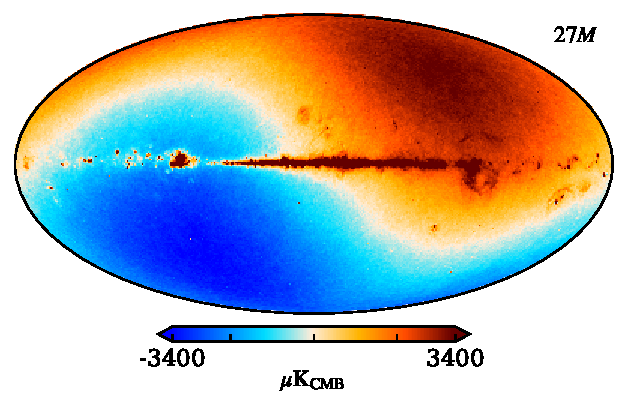
\includegraphics[width=0.49\textwidth]{figs/sim_T_27M.pdf}
  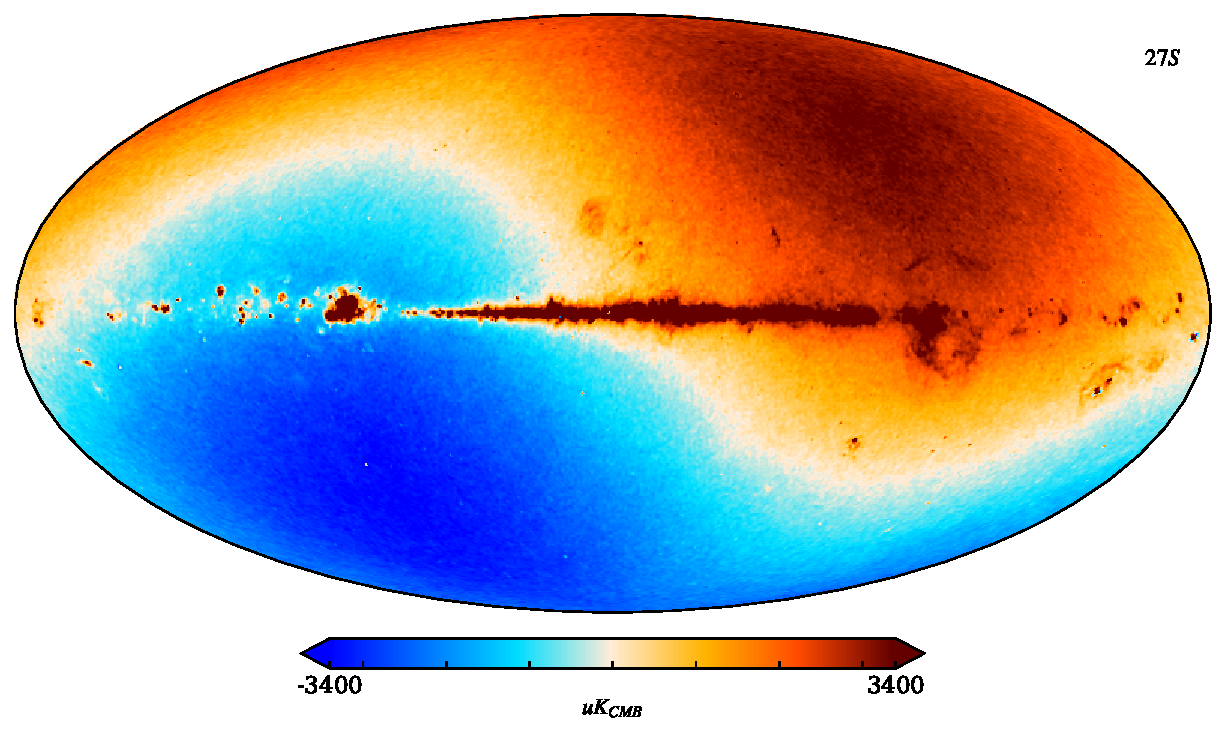
\includegraphics[width=0.49\textwidth]{figs/sim_T_27S.pdf}\\
  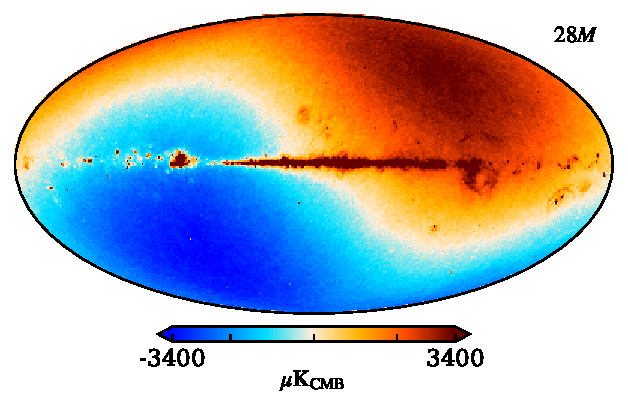
\includegraphics[width=0.49\textwidth]{figs/sim_T_28M.pdf}
  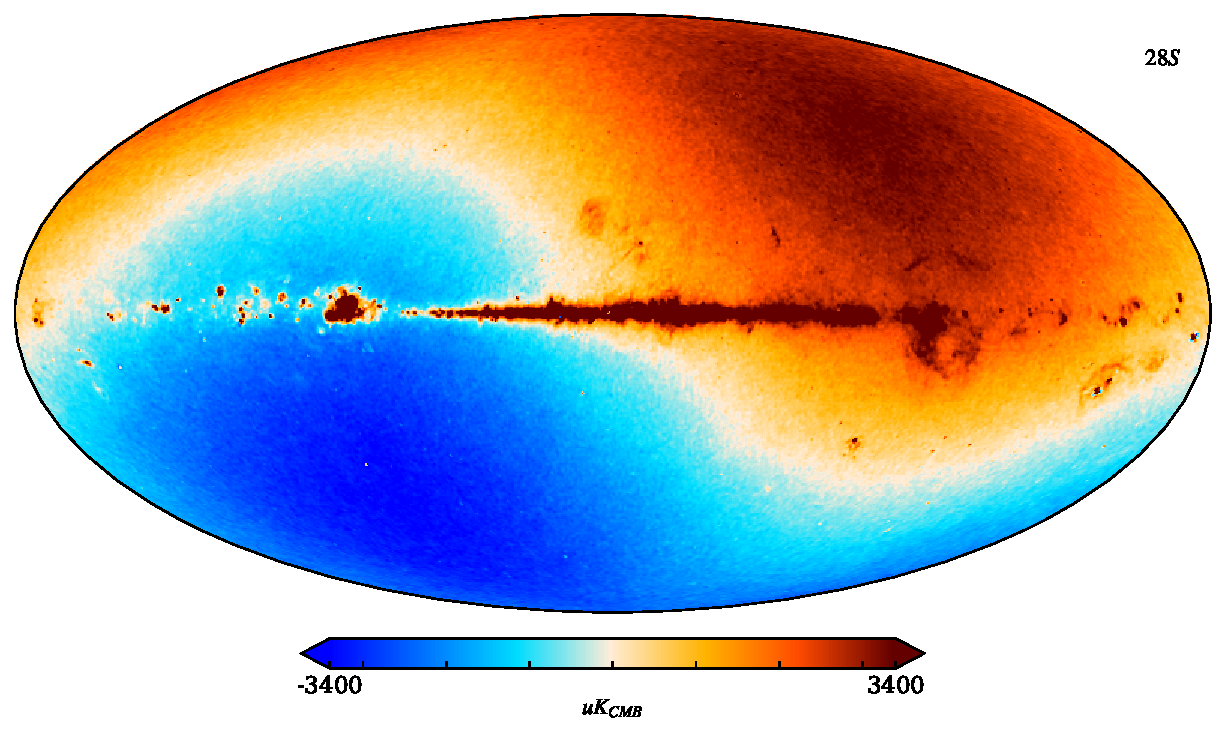
\includegraphics[width=0.49\textwidth]{figs/sim_T_28S.pdf}\\
  %\includegraphics[width=0.5\columnwidth]{figs/cbar_temp.pdf}\\
  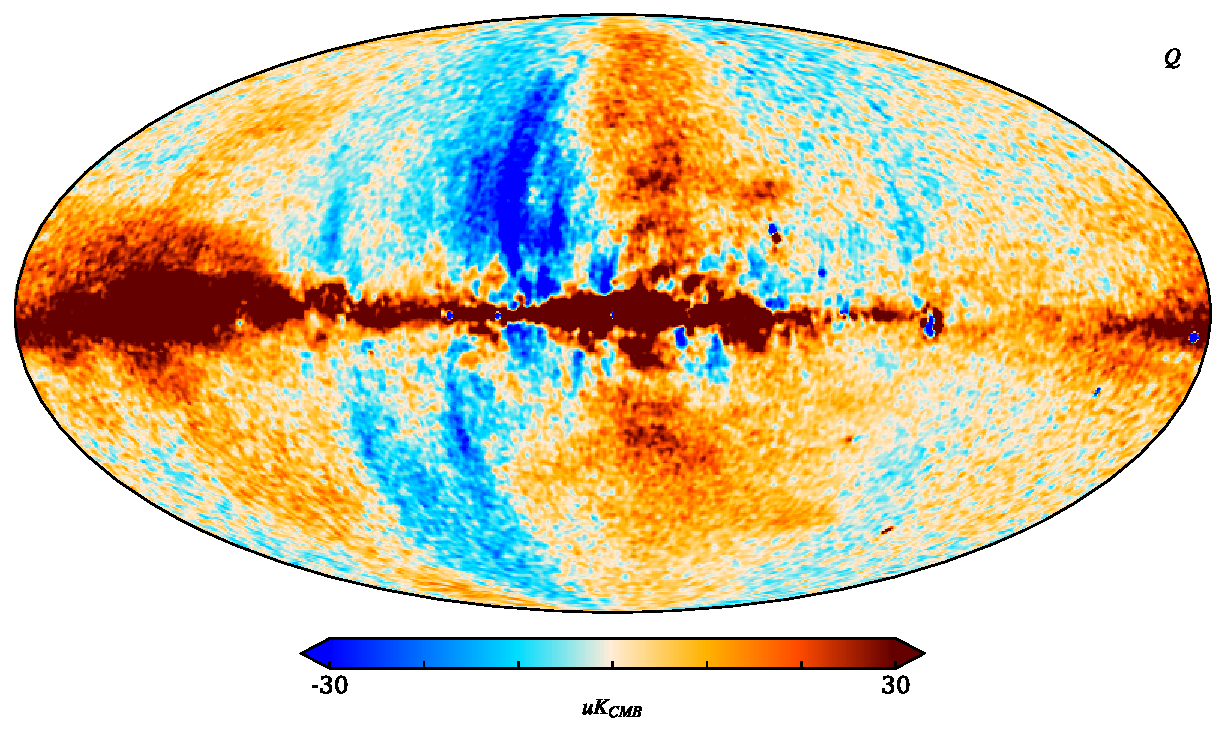
\includegraphics[width=0.49\textwidth]{figs/sim_Q.pdf}
  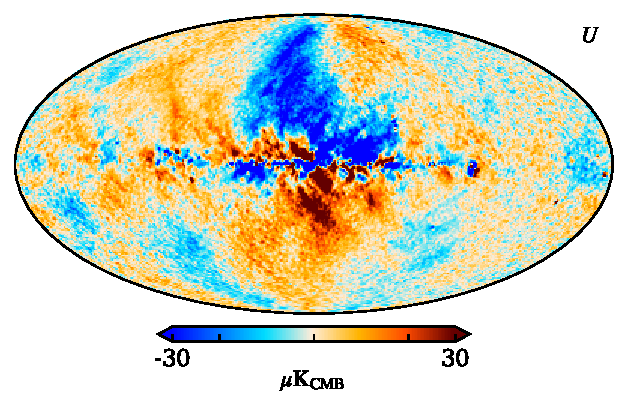
\includegraphics[width=0.49\textwidth]{figs/sim_U.pdf}\\
  %\includegraphics[width=0.5\columnwidth]{figs/cbar_pol.pdf}\\
  \caption{Simulated temperature and polarization maps of the LFI 30\,GHz data produced using $N+2$ mapmaking. The top four panels show the temperature maps, and the bottom row shows the combined $Q$ and $U$ maps.}
  \label{fig:sim}
\end{figure*}

\begin{figure*}
  \centering
  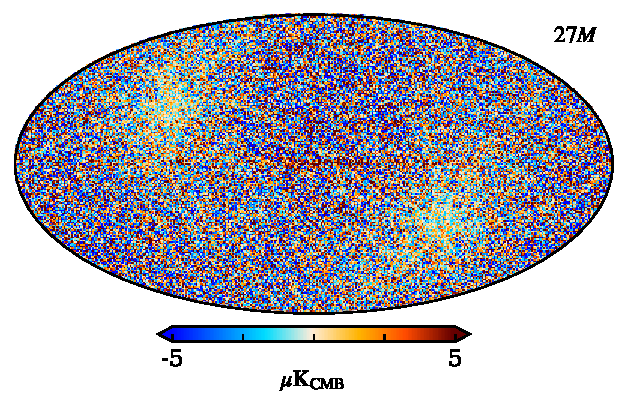
\includegraphics[width=0.49\textwidth]{figs/sim_diff_T_27M.pdf}
  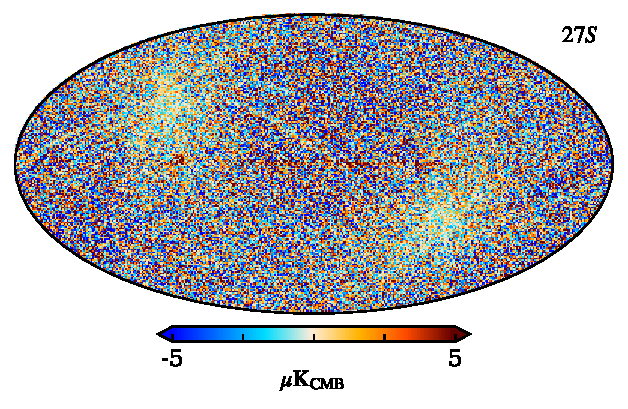
\includegraphics[width=0.49\textwidth]{figs/sim_diff_T_27S.pdf}\\
  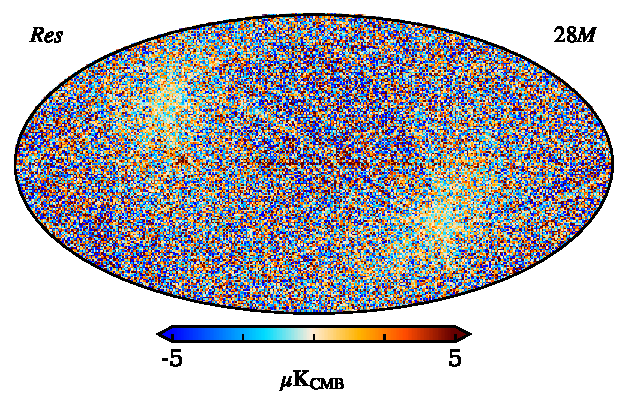
\includegraphics[width=0.49\textwidth]{figs/sim_diff_T_28M.pdf}
  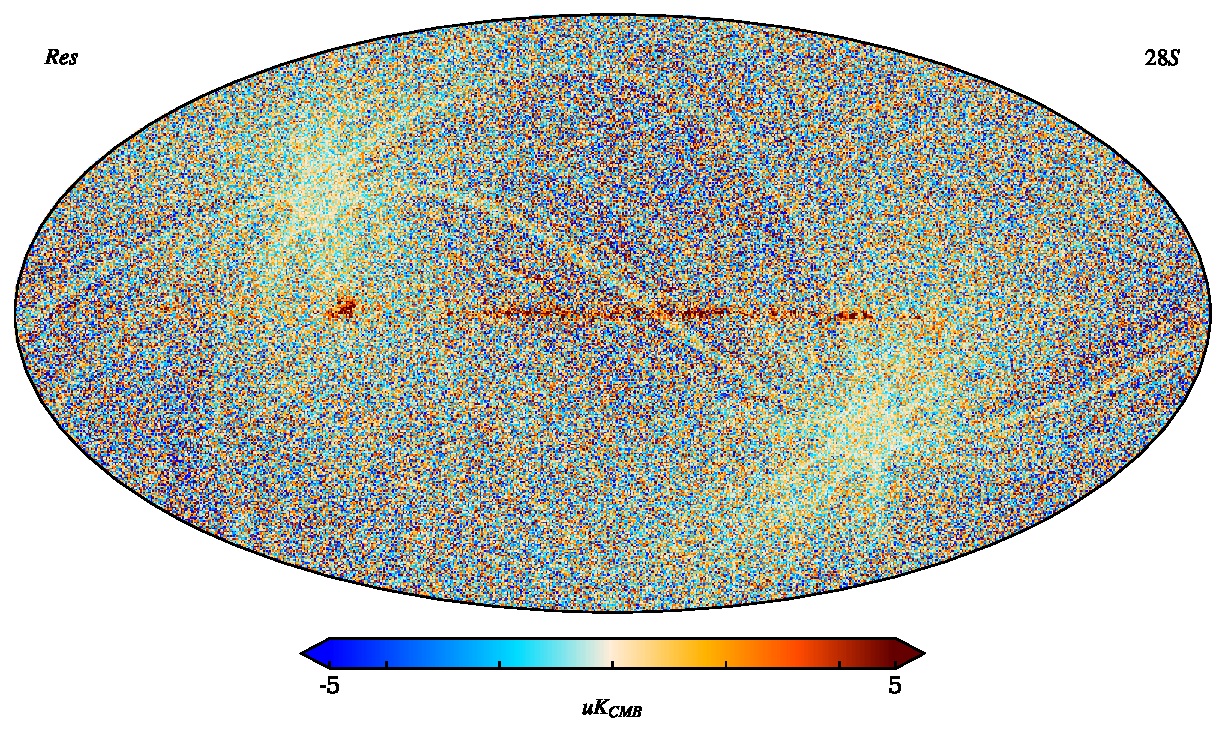
\includegraphics[width=0.49\textwidth]{figs/sim_diff_T_28S.pdf}\\
  %\includegraphics[width=0.5\columnwidth]{figs/cbar_temp.pdf}\\
  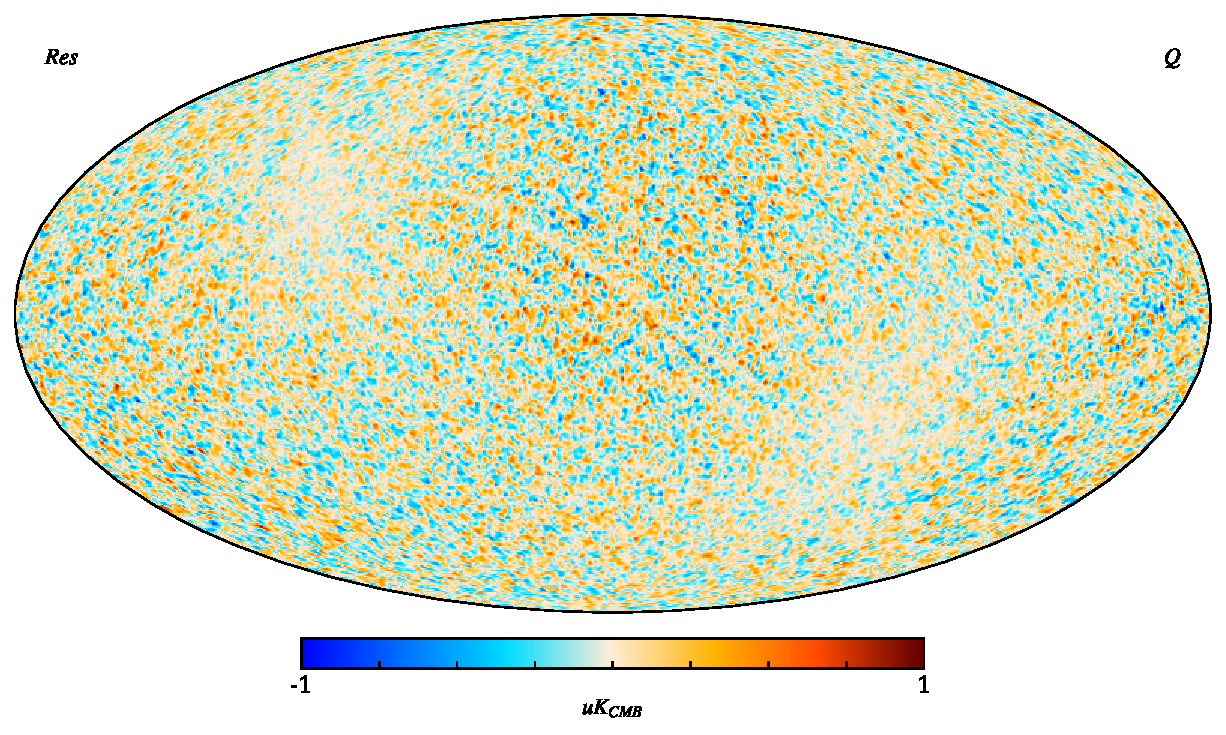
\includegraphics[width=0.49\textwidth]{figs/sim_diff_Q.pdf}
  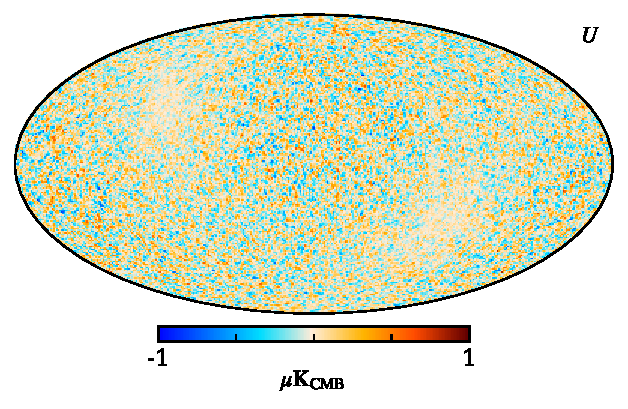
\includegraphics[width=0.49\textwidth]{figs/sim_diff_U.pdf}\\
  %\includegraphics[width=0.5\columnwidth]{figs/cbar_pol.pdf}\\
  \caption{Input sky minus output maps for the simulated LFI 30\,GHz sky as generated using $N+2$ mapmaking in \commanderthree\. The top four panels show the temperature maps, and the bottom row shows the combined $Q$ and $U$ maps.}
  \label{fig:sim_diff}
\end{figure*}



%\begin{figure*}
%\begin{tabular}{B C C C}
%& 27S & 28M & 28S\\  
%  27M & 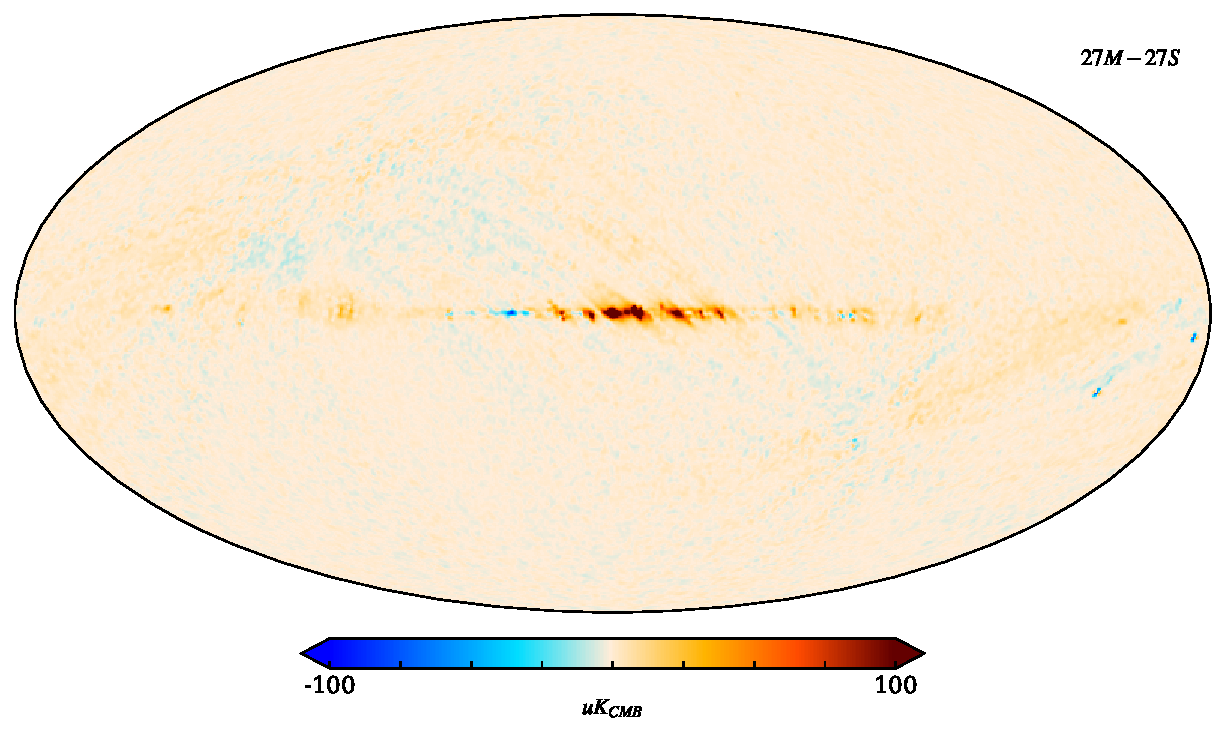
\includegraphics[width=0.31\textwidth]{figs/27M_minus_27S_depol.pdf} & 
%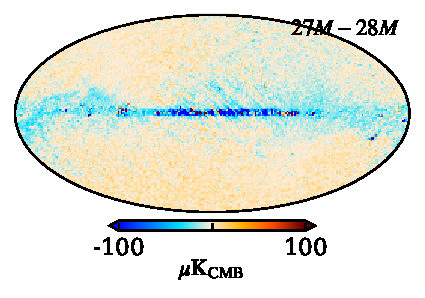
\includegraphics[width=0.31\textwidth]{figs/27M_minus_28M_depol.pdf} &
%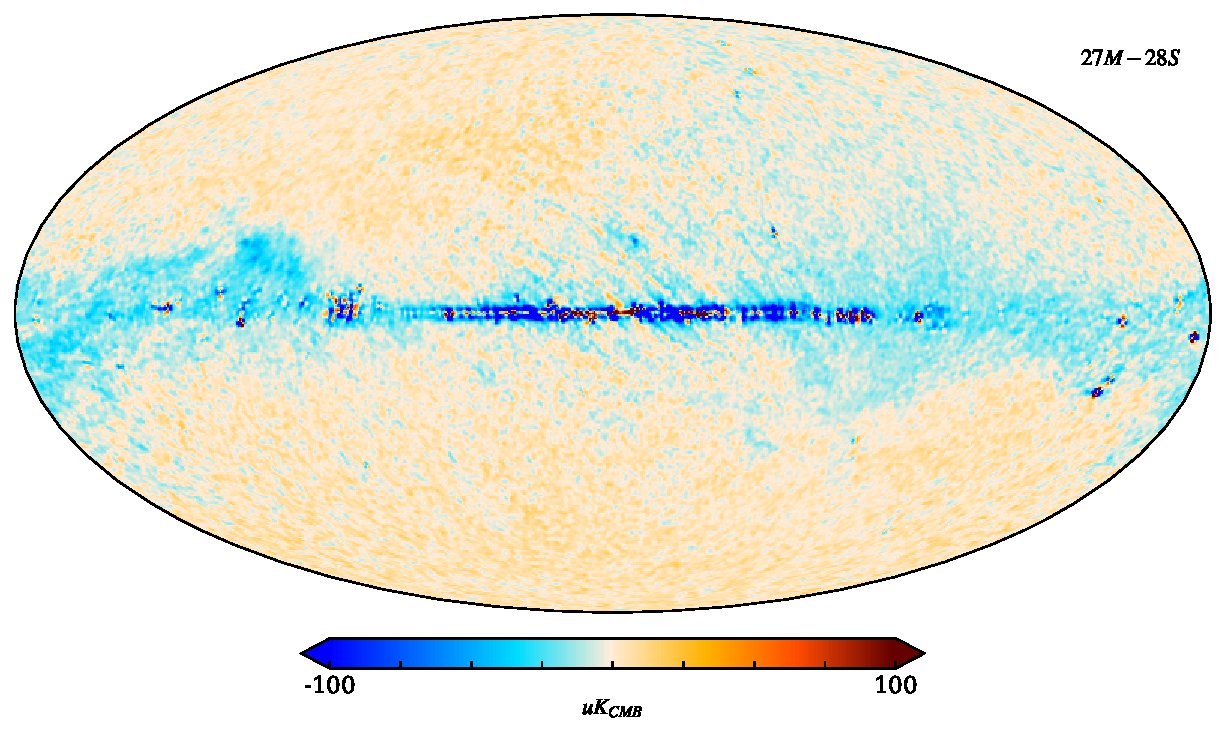
\includegraphics[width=0.31\textwidth]{figs/27M_minus_28S_depol.pdf}\\
% & \hspace{4.8cm } 27S & 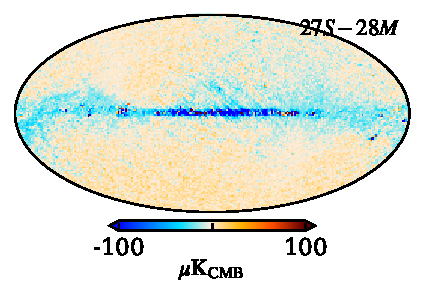
\includegraphics[width=0.31\textwidth]{figs/27S_minus_28M_depol.pdf} &
% 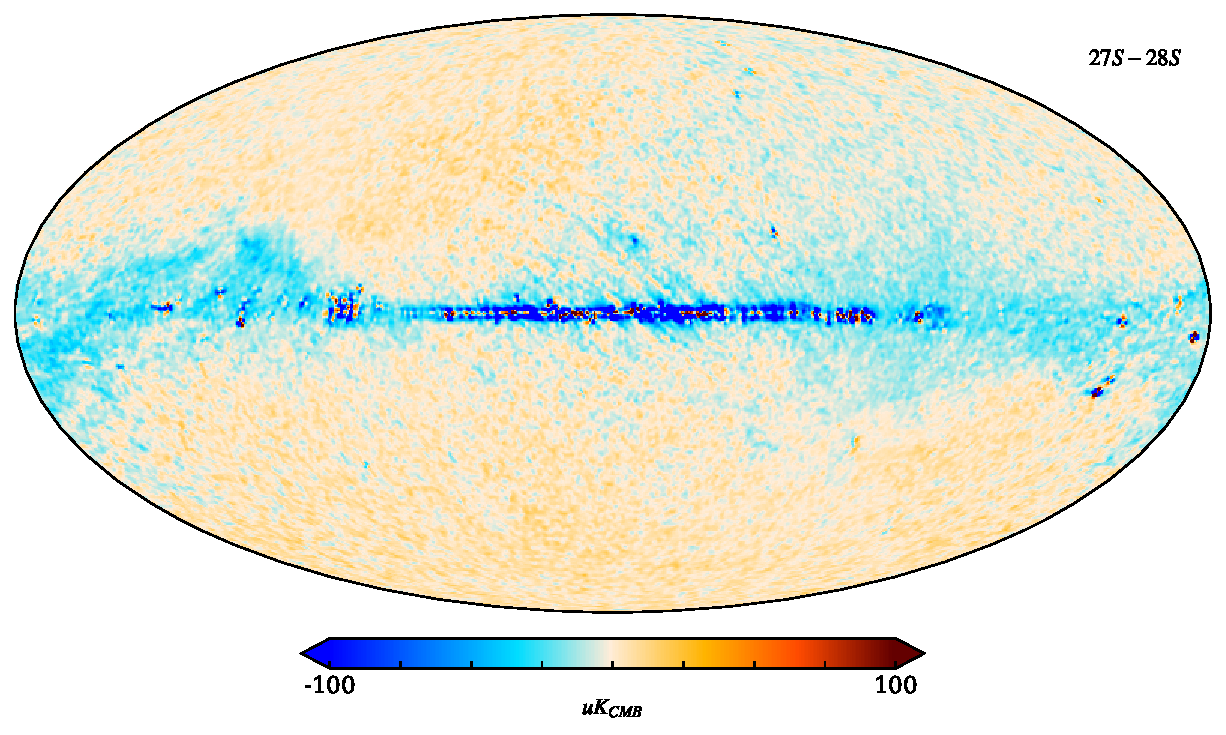
\includegraphics[width=0.31\textwidth]{figs/27S_minus_28S_depol.pdf}\\
% &     \caption{All 6 possible difference maps between the 30 Ghz detectors. }   \label{fig:bp_diffs} & \hspace{4.7cm } 28M  & 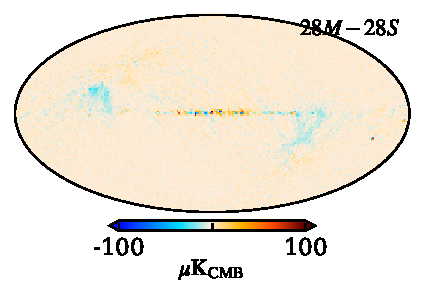
\includegraphics[width=0.31\textwidth]{figs/28M_minus_28S_depol.pdf} \\
%  %\includegraphics[width=0.5\columnwidth]{figs/cbar_pol.pdf}\\
%  \end{tabular}
%\vspace{-0.75cm}
%\end{figure*}





To understand the behaviour of the new $N+2$ mapmaking algorithm, we start by applying it to a well-known case, namely the \Planck\ LFI 30\,GHz data. In particular, we implement this algorithm within the Bayesian \commanderthree\ \citep{bp03} Gibbs sampling code developed by the \BP\ and \cosmoglobe\ collaborations \citep{bp01, watts2023_dr1}, and the raw TOD data are processed in an identical manner as in those works with respect to calibration, correlated noise etc. Only the signal-plus-white noise residual TOD are fed to the $N+2$ mapmaker, and our new contribution thus replaces the full-frequency binned mapmaker presented by \citet{BP10}. 

To briefly summarize this general algorithmic approach, we start by defining a single parametric model for both the sky and instrument, and for LFI this is currently given by
\begin{equation}
  \begin{split}
    d_{j,t} = g_{j,t}&\tens{P}_{tp,j}\left[\tens{B}^{\mathrm{symm}}_{pp',j}\sum_{c}
      \tens{M}_{cj}(\beta_{p'}, \Delta_{\mathrm{bp}})a^c_{p'}  + \tens{B}^{\mathrm{asymm}}_{j,t}\left(\vec{s}^{\mathrm{orb}}_{j}  
      + \vec{s}^{\mathrm{fsl}}_{t}\right)\right] + \\
%    + s^{\mathrm{fsl}}_{j,t} + s^{\mathrm{mono}}_{j}\right] + \\
    + &n^{\mathrm{corr}}_{j,t} + n^{\mathrm{w}}_{j,t}.
  \end{split}
  \label{eq:todmodel}
\end{equation}
The details of this model are discussed in \citep{bp01}, but we note that the terms directly relevant to mapmaking are the pointing matrix $\tens{P}_{tp,j}$; the sky signal, which is the sum over sky components $\sum_{c} \tens{M}_{cj}(\beta_{p'}, \Delta_{\mathrm{bp}})a^c_{p'}$; and the white noise $n^{\mathrm{w}}_{j,t}$. The rest of the terms (like the sidelobes or correlated noise) are allowed by the Gibbs sampling algorithm \citep{gibbs} to be assumed fixed during mapmaking, and thus can be treated as deterministic contaminants and removed as a pre-processing step. This approach greatly simplifies the formal mapmaking process, as we do not need to mitigate correlated noise or other systematics during mapmaking, and can simply bin the TOD per pixel to average down the white noise, using the approach detailed in Sect.~\ref{sec:mapmaking}.

Applying this method to the four LFI 30\,GHz detectors (denoted 27M, 27S, 28M, and 28S, respectively), the $N+2$ mapmaker produces four distinct temperature maps, shown in the first and second rows, in addition to combined $Q$ and $U$ maps, shown in the third row. These maps can be seen in Fig.~\ref{fig:maps}. For comparison, the bottom row shows the corresponding $Q$ and $U$ maps produced from the traditional binned mapmaker, which have been extensively verified by multiple implementations of the algorithm over many years \citep[e.g.,][]{lfi2013,lfi2015,lfi2018}. Comparing the maps in the third and fourth rows in Fig.~\ref{fig:maps}, we see already at a purely visual level that the new $N+2$ mapmaker does not produce maps that are competitive with the traditional approach for the \Planck\ 30\,GHz data, neither in terms of overall noise levels nor temperature-to-polarization leakage. We investigate the origin of this problem in the next section.

\subsection{Polarization Angle Coverage}

The root cause of the polarization problems seen in Fig.~\ref{fig:maps} is the limited polarization angle coverage of the \Planck\ scanning strategy. When the \Planck\ mission was originally designed, it was optimized for thermal stability with respect to intensity reconstruction, which resulted a scan path following nearly great circles in Ecliptic coordinates, modulated by a slow cycloidal procession to improve coverage at the ecliptic poles \citep{planckScan}. While this scanning strategy did ensure that the \Planck\ instrument could meet its thermal requirements, it also had unfortunately consequences for polarization reconstruction. The main problem is simply that each detector sees each pixel on the sky with a very limited range of polarization angles, $\phi$. This, in turn, results in a poorly conditioned matrix $\A^t\N^{-1}\A$, as defined in Sect.~\ref{sec:mapmaking}. This is visualized in Fig.~\ref{fig:polangles}, where we plot the off-diagonal temperature-polarization cross terms, $(\frac{1}{\sigma_i})^2 \cos2\phi_i$ and $(\frac{1}{\sigma_i})^2 \sin2\phi_i$, for the four 30\,GHz detectors in the top four rows. For comparison, the bottom row shows the same quantity for the full co-added frequency channel map, which corresponds to the traditional binned mapmaker. 

For an experiment with a perfectly uniform polarization coverage, these maps are consistent with zero, as the sine and cosine terms cancel when averaged over the polarization angle $\phi$. As a result, the coupling matrix, $\A^t\N^{-1}\A$, becomes diagonal, and the overall condition number is defined by the noise level alone. For the \Planck\ scanning strategy, this is not the case. Rather, we immediately see from the bottom row in Fig.~\ref{fig:polangles} that the magnitude of the coadded coupling matrix is almost an order of magnitude smaller than any of the individual detectors. Even worse, we also note that pairs of detectors, such as 28M and 28S, have a very similar spatial morphology, but with opposite signs. As a result, the mean condition number of the per-detector coupling matrix is about 100, while it is about 2 for the co-added case. This means effectively that the white noise variance of the individual detector maps is boosted by a factor of 50, and this is what is seen visually in the bottom two rows of Fig.~\ref{fig:maps}. In practice, this means that the $N+2$ mapmaking algorithm is not immediately useful for \Planck\ in its most direct way. On the other hand, these calculations do also suggest that building horn maps (by coadding pairs of detectors within a single horn) may be a viable strategy for future analysis.

\subsection{Simulations with a spinning half-wave plate}
\label{sec:sim}

Next, we apply the $N+2$ mapmaker to a case with nearly perfect polarization angle coverage, by replacing the real LFI 30\,GHz data above with a \commanderthree-based TOD simulation, as described in \commanderthree\ \citep{BP04}. Intuitively speaking, this amounts to replacing the real data with a random realization drawn from the data model described by Eq.~\ref{eq:todmodel}. However, to mitigate the poor polarization coverage discussed above, we replace the polarization angle in each sample with a random orientation, which essentially corresponds to adding an ideal infinitely fast spinning half-wave plate to the \Planck\ optical system. The resulting maps are shown in Fig.~\ref{fig:sim}, and the corresponding differences with respect to the (now true known) input sky map is shown in Fig.~\ref{fig:sim_diff}. With this modification, we see a low-amplitude residual along the Galactic plane in temperature at the level of $\mathcal{O}(10^{-4})$; because there is a finite number of samples hitting each pixel, the off-diagonal coupling matrix is not perfectly zero, and a small level of bandpass-induced temperature-to-polarization leakage therefore still leaks through in the very brightest foreground emission parts of the sky. However, both the rest of the temperature maps and the polarization maps are all consistent with noise, and this demonstrates that the $N+2$ algorithm does work as intended.

\section{Bandpass reconstruction and leakage mitigation}

\begin{figure*}
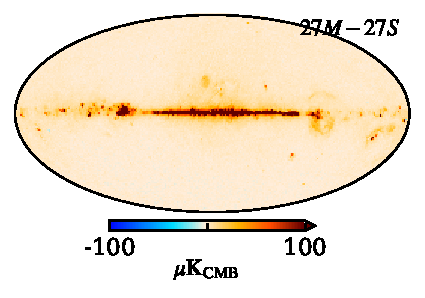
\includegraphics[width=0.31\textwidth]{figs/sim_27M_minus_27S.pdf} 
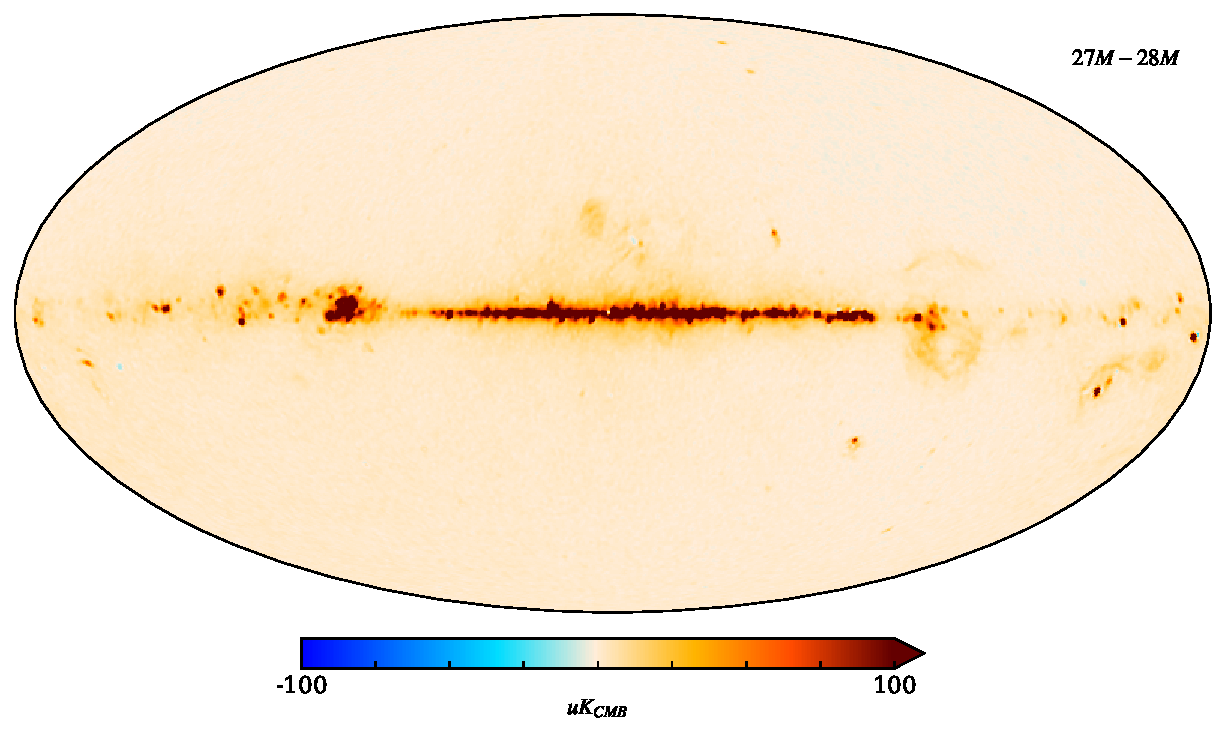
\includegraphics[width=0.31\textwidth]{figs/sim_27M_minus_28M.pdf} 
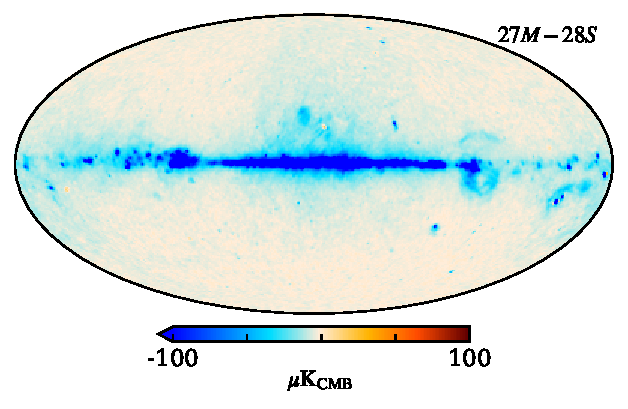
\includegraphics[width=0.31\textwidth]{figs/sim_27M_minus_28S.pdf}\\
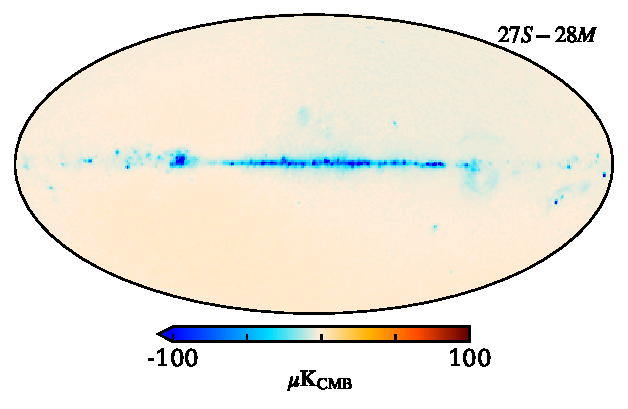
\includegraphics[width=0.31\textwidth]{figs/sim_27S_minus_28M.pdf} 
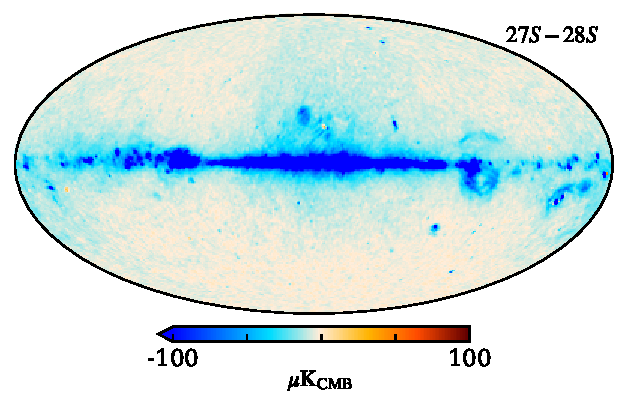
\includegraphics[width=0.31\textwidth]{figs/sim_27S_minus_28S.pdf}
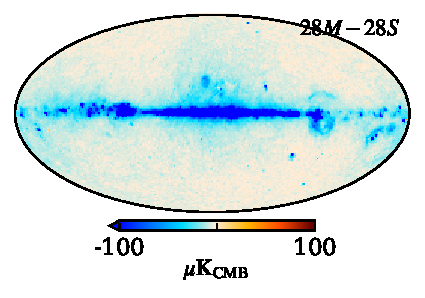
\includegraphics[width=0.31\textwidth]{figs/sim_28M_minus_28S.pdf}
\caption{All 6 possible difference maps between the simulated 30 GHz maps. 
	{\bf I can help with the formatting of these. (DW)}
	} \label{fig:sim_bp_diffs}
\end{figure*}


\begin{figure}[]
\includegraphics[width=\linewidth]{figs/map_Q_leak_comp.pdf}\\
\includegraphics[width=\linewidth]{figs/map_Q_leak_nplus2_comp.pdf}
\caption{Comparison of temperature-to-polarization leakage for a constant monopole term as processed through a standard co-adding mapmaker (top panel) and through the $N+2$ mapmaker (bottom panel). Note the different colour scales.}
\label{fig:leak}
\end{figure}

The original motivation for considering the $N+2$ mapmaking idea was twofold: firstly, the separation of the temperature maps for each detector improves our ability to perform component separation in the case of differing bandpasses, in particular for line emission components, and secondly that it helps mitigate temperature-to-polarization leakage caused by bandpass differences. To illustrate the first effect, Fig.~\ref{fig:sim_bp_diffs} shows pairwise temperature difference maps between the simulated temperature maps discussed above. We see that, for each case, the difference between channels $A$ and $B$ clearly exhibits the morphology of the Galactic plane, with an overall uniform color range; red if the effective central frequency for channel $A$ is lower than for channel $B$, and blue otherwise. This sign depends on the slope of the spectral energy density of the dominant foreground component in the Galaxy, which at 30\,GHz is synchrotron emission. This is stronger at lower frequencies, and a lower central frequency therefore implies a stronger signal. These bandpass differences are precisely the effects that we want capture with separate temperature maps.

To illustrate the second advantage, namely the capability of mitigating temperature-to-polarization leakage, we create yet another simulation of the same type as above (including polarization angle randomization), but this time we inject a bright artificial offset into one of the four 30\,GHz detectors, with an amplitude of 1\,mK. The signal is unpolarized, as it is added uniformly to each sample for the given detector, and therefore represents a detector-specific temperature excess. As a result, it will introduce temperature-to-polarization leakage, similar to for instance traditional bandpass, beam or gain mismatches. The top panel of Fig.~\ref{fig:leak} shows the Stokes $Q$ leakage map induced by this contribution when applying the traditional co-addition mapmaker, evaluated by subtracting the frequency maps derived with and without the spurious terms. For comparison, the bottom panel shows the same map when applying the $N+2$ mapmaker. The leakage amplitude in the second case is more than six orders of magnitude fainter. 

\section{Conclusions and Future Plans}
\label{sec:conclusions}

We have introduced $N+2$ mapmaking as a novel method producing temperature and polarization maps from multi-detector CMB timestreams. The motivation behind this method is two-fold; it allows the user to produce single-detector temperature maps from polarized TOD, which are useful for component separation purposes. Secondly, it helps mitigating various temperature-to-polarization leakage effects, for instance bandpass mismatch. Algorithmically speaking, this method is very closely related to the `spurious mapmaking' approach introduced by the \WMAP\ team, but rather than solving for $N-1$ residual maps, we solve directly for $N$ physically meaningful temperature maps. Indeed, the $N+2$ mapmaking algorithm was originally developed in preparation for a future Bayesian analysis of the \Planck\ HFI data, in which both leakage and CO line emimssion are important effects. This work is organized within the OpenHFI initiative, which is a sub-group of the Cosmoglobe collaboration. The next step in this process is to integrate the $N+2$ concept into an iterative Conjugate Gradient solver that simultaneously accounts for the HFI bolometer transfer function as demonstrated by \cite{artem}. 

In the current paper, we apply the $N+2$ formalism to the \Planck\ LFI 30\,GHz data within the Bayesian \commanderthree\ framework, at first attempting to produce single-detector temperature maps jointly with coadded polarization maps. Unfortunately, we find that poor polarization angle coverage of the \Planck\ scanning strategy prohibits a robust separation of temperature and polarization signals. In future work, it is therefore instead worth considering producing horn maps, as for instance done in \Planck\ PR4 \citep{npipe}. However, in that work the horn maps were produced as a post-processing step that was separate from the main analysis, whereas with the new $N+2$ mapmaker the horn maps can be derived jointly with the co-added polarization maps. This is particularly useful in within an iterative end-to-end Bayesian framework like \Cosmoglobe, in which close interaction between the calibration, mapmaking and component separation steps is essential.    

When applying the $N+2$ algorithm to a simulated LFI-like data set with randomized polarization angles, corresponding to adding a fast rotating half-wave plate to the instrument, we find that the $N+2$ algorithm produces maps that consistent with expectations. In this case, we also find that the algorithm is capable of producing single-detector temperature maps with minimal temperature-to-polarization leakage. Incidentally, based on the same test, we also show that the introduction of a spinning half-wave plate does not by itself allow the production of clean polarization maps from multi-detector observations, which is of interest for future experiments that rely on a spinning half-wave plate, such as LiteBIRD \citep{litebird2022}. For these, the $N+2$ mapmaking algorithm offers the possibility of making multi-detector maps with effective tempeature-to-polarization leakage as an alternative to the standard single-detector maps. This could be useful for mitigating correlated but low signal-to-noise ratio systematic effects that would benefit from detector coaddition. 

\begin{acknowledgements}
 The current work has received funding from the European
  Union’s Horizon 2020 research and innovation programme under grant
  agreement numbers 819478 (ERC; \textsc{Cosmoglobe}) and 772253 (ERC;
  \textsc{bits2cosmology}). Some of the results in this paper have been derived using the HEALPix \citep{healpix} package.
  We acknowledge the use of the Legacy Archive for Microwave Background Data
  Analysis (LAMBDA), part of the High Energy Astrophysics Science Archive Center
  (HEASARC). HEASARC/LAMBDA is a service of the Astrophysics Science Division at
  the NASA Goddard Space Flight Center.  
\end{acknowledgements}


%-------------------------------------------------------------
%                                       Table with references 
%-------------------------------------------------------------
%

\bibliographystyle{aa}
\bibliography{references, ../../common/CG_bibliography}
\end{document}
%%%% End of aa.dem



\subsection{Depolarized mapmaking}
\label{sec:depol}



%\begin{figure*}[t]
%  \centering
%  \includegraphics[width=0.49\textwidth]{figs/map_T_27M_depol.pdf}
%  \includegraphics[width=0.49\textwidth]{figs/map_T_27S_depol.pdf}\\
%  \includegraphics[width=0.49\textwidth]{figs/map_T_28M_depol.pdf}
%  \includegraphics[width=0.49\textwidth]{figs/map_T_28S_depol.pdf}\\
%  %\includegraphics[width=0.5\columnwidth]{figs/cbar_temp.pdf}\\
%  \includegraphics[width=0.49\textwidth]{figs/map_Q_depol.pdf}
%  \includegraphics[width=0.49\textwidth]{figs/map_U_depol.pdf}\\
%  %\includegraphics[width=0.5\columnwidth]{figs/cbar_pol.pdf}\\
%  \caption{Temperature and polarization maps of the LFI 30 GHz data produced using depolarized n+2 mapmaking. The top four panels contain the temperature maps, and the bottom row contains the combined Q and U maps.}
%  \label{fig:depolarized}
%\end{figure*}



It is still possible, to simultaneously produce individual temperature maps and joint polarization maps in this case, albeit without all of the nice leakage-reducing properties of the ideal N+2 mapmaker. To generate our Q and U polarization maps in this case, we are forced to construct a traditional 3x3 $A^t N^{-1}A$ matrix, of the form

\begin{equation}
\begin{pmatrix}
(\frac{1}{\sigma})^2 &
(\frac{1}{\sigma})^2 \cos2\phi_t & (\frac{1}{\sigma})^2 \sin2\phi_t \\

(\frac{1}{\sigma})^2 \cos2\phi_t & 
(\frac{\cos 2\phi_t}{\sigma})^2 & (\frac{1}{\sigma})^2 \sin2\phi_t \cos2\phi_t \\

(\frac{1}{\sigma})^2 \sin2\phi_t & 
(\frac{1}{\sigma})^2 \sin2\phi_t \cos2\phi_t &(\frac{ \sin 2\phi_t}{\sigma})^2
\\
\end{pmatrix}
.
\end{equation}

Here, each entry includes contributions from every detector. We can then compute the GLS solution to Eq. \ref{eq:gls} and solve for our common sky signal vector 

\begin{equation}
S_p = \begin{pmatrix}
I_p\\
Q_p\\
U_p\\
\end{pmatrix}.
\end{equation}

Once we have derived $Q$ and $U$ for our pixel $p$, the temperature data as a function of time and pixel follows from the data model of eq. \ref{eq:datamodel}. 

\begin{equation}
T_{i,p} = d_{i,p,t} - Q_p \cos2\phi_t - U_p \sin2\phi_t.
\end{equation}


$Q_p$ and $U_p$ are given by the sky vector we solved for with the 3x3 case, and so to compute the depolarized temperature map for each detector we can simply perform a noise weighted sum over the time index $t$ for each pixel $p$. The quantities $\sum_t d_{i,p,t}/\sigma_t^2$, $\sum_t \cos2\phi_t/\sigma_t^2$ and $\sum_t \sin2\phi_t/\sigma_t^2$ have already been precomputed as elements of the N+2 mapmaking matrix, and so it is trivial to then solve for the depolarized temperature maps given the polarized components. 

These maps are shown in fig. \ref{fig:depolarized} for LFI 30GHz, and it is clear that this method produces a better result than that of the previous approach. The polarized maps are identical to those of the 3x3 binned mapmaker, but this approach maintains the additional advantage of producing the individual temperature maps.

Figure \ref{fig:bp_diffs} shows the 6 possible difference maps between these four temperature maps, smoothed to one degree to show their structure. These differences are largest in the galactic plane, where signals amplitudes are highest. We see that in this simulation the 28S detector is somewhat of an outlier, which does not match the real data perfectly, but overall, the amplitudes are low, and are easily explained by bandpass differences between detector pairs.


\begin{figure*}
\begin{tabular}{B C C C}
& 27S & 28M & 28S\\
  27M & \includegraphics[width=0.30\textwidth]{figs/sim_27M_minus_27S.pdf} & 
\includegraphics[width=0.30\textwidth]{figs/sim_27M_minus_28M.pdf} &
\includegraphics[width=0.31\textwidth]{figs/sim_27M_minus_28S.pdf}\\
 & \hspace{4.8cm } 27S & \includegraphics[width=0.31\textwidth]{figs/sim_27S_minus_28M.pdf} &
 \includegraphics[width=0.31\textwidth]{figs/sim_27S_minus_28S.pdf}\\
 & \caption{All 6 possible difference maps between the simulated 30 GHz maps. 

	} \label{fig:sim_bp_diffs} &  \hspace{4.7cm }  28M  & \includegraphics[width=0.31\textwidth]{figs/sim_28M_minus_28S.pdf} \\
  %\includegraphics[width=0.5\columnwidth]{figs/cbar_pol.pdf}\\
  \end{tabular}
\vspace{-0.75cm}
\end{figure*}
